\chapter{Регулярные задачи стохастического управления с конечным топливом} \label{chapt2}

\section{Введение}\label{sec:2.1}
Рассмотрим задачу управления, в которой требуется как можно дольше удерживать стохастическую систему $X$ в заданной области $G$. Воздействие на систему $X$ требует расхода ресурса (или топлива). Задача состоит в том, чтобы использовать имеющееся количество ресурса оптимальным образом.

Изучение диффузионных стохастических задач управления с конечным топливом было начато в \cite{BatChe67b}, где рассматривалась задача о приближении космического аппарата к случайной цели. Впоследствии задачи с конечным топливом разрабатывались почти исключительно в парадигме сингулярного стохастического управления \cite{BatChe67a,BatChe67b}. При этом подходе всегда оптимально удерживать систему в так называемой <<области бездействия>>. Существенный шаг был сделан в \cite{BenSheWit1980}. В указанной статье изучалась задача оптимального отслеживания броуновского движения процессом, вариация которого ограничена заданным начальным запасом топлива. Было получено явное решение для квадратического дисконтированного критерия в случае бесконечного горизонта. В частности, было отмечено, что оптимальная область бездействия расширяется с уменьшением количества доступного топлива.

Более общие задачи такого рода изучались впоследствии, например, в \cite{KarShr86,BriShr92,KarOcoWanZer00}. Случай конечного горизонта рассмотрен, в работах \cite{Kar85,ChoMenRob85,ElKKar88}. Весьма общие результаты, касающиеся характеризации функции Беллмана и существование оптимальных стратегий управления, были получены в \cite{DufMil02,MotSar07,MotSar08a,MotSar08b}. Многие работы были мотивированы приложениями. Отметим задачи оптимальной коррекции движения \cite{Che71}, управления спутником \cite{Jac83,Jac99,Jac02}, достижения цели игроком \cite{SudWee92,Wee92}, оптимальной ликвидации и
оптимального исполнения транзакций \cite{PemZhaYin07,GatSch11,BiaWuZhe14,BecBilFre15}.

В отличие от подавляющего большинства известных работ, мы предполагаем что интенсивность потребления ресурса (топлива) ограничена. Фактически, только \cite{PemZhaYin07,BiaWuZhe14} из перечисленных выше работ используют аналогичное предположение. Ограничиваясь классическими управлениями, мы приходим к более простым математическим задачам, которые, тем не менее, способны описывать интересные эффекты и имеют широкий диапазон возможных приложений. С формальной точки зрения мы работаем с нелинейным параболическим уравнением Гамильтона-Якоби-Беллмана (Hamiltnon-Jacobi-Bellman: HJB) и классическими управлениями, вместо вариационного неравенства и сингулярных управлений. Несмотря на эти отличия, в обоих случаях в фазовом пространстве имеется область бездействия $\Pi_{na}$. Когда фазовая переменная находится в этой области оптимальная стратегия состоит в том, чтобы не расходовать топливо. Сингулярные управления способны удерживать систему в области $\Pi_{na}$. Используемые нами классические управления лишь создают снос в сторону $\Pi_{na}$.

Для того, чтобы дать точную формулировку нашей задачи рассмотрим стандартный $m$-размерный винеровский процесс  $W=(W^1,\dots W^m)$, определенный на вероятностном пространстве $(\Omega,\mathcal F,\mathsf P)$, где $\mathbb F=(\mathscr F_s)_{s\ge 0}$ --- минимальная пополненная естественная фильтрация процесса $W$. Пусть управляемый процесс $X=(X^1,\dots,X^d)$ подчиняется системе стохастических дифференциальных уравнений
\begin{equation} \label{eq:2.1.1}
dX_t=b(X_t,\alpha_t) dt+\sigma(X_t,\alpha_t) dW_t, \quad X_0=x.
\end{equation}
Входящий сюда $\mathbb F$-прогрессивно измеримый процесс $\alpha \in A=[\underline a, \overline a]$, $\underline a\le 0\le \overline a$ можно рассматривать как интенсивность потребления ресурса. Мы предполагаем что компоненты вектора сноса $b:\mathbb R^d\times A\mapsto\mathbb R^d$ и матрицы диффузии $\sigma:\mathbb R^d\times A\mapsto\mathbb R^d\times\mathbb R^m$ непрерывны и удовлетворяют неравенству
$$|b(x,a)-b(y,a)|+|\sigma(x,a)-\sigma(y,a)|\le K|x-y|,$$
где константа $K$ не зависит от $a$. Заметим ,что это неравенство влечет также условие линейного роста:
$$ |b(x,a)|+|\sigma(x,a)|\le K'(1+|x|).$$
Таким образом, существует единственное $\mathbb F$-согласованное сильное решение (\ref{eq:2.1.1}) на $[0,\infty)$: см. \cite{Kry80} (Глава 2). Количество ресурса $Y$ удовлетворяет уравнению
\begin{equation} \label{eq:2.1.2}
dY_t=-|\alpha_t|dt,\quad Y_0=y.
\end{equation}

Процесс $\alpha$ назовем \emph{допустимым}, и будем использовать обозначение $\alpha \in \mathcal A(x,y)$, если $Y_t \ge 0$, $t\ge 0$. Допустимость означает, что перерасход ресурса запрещен. Решение (\ref{eq:2.1.1}), (\ref{eq:2.1.2}) обозначим через $X^{x,y,\alpha}, Y^{x,y,\alpha}$.

Пусть $G\subset \mathbb R^d$ открытое множество. Нам будет удобно предположить, что $0\in G$. В общем случае мы не накладываем на $G$ условия ограниченности. Обозначим через
$\theta^{x,y,\alpha}=\inf\{t\ge 0:X_t^{x,y,\alpha}\not \in G\}$ время выхода процесса $X^{x,y,\alpha}$ из области $G$.
Определим целевой функционал $J$ и функцию Беллмана $v$ следующим образом:
\begin{equation} \label{eq:2.1.3}
J(x,y,\alpha)=\mathsf E\int_0^{\theta^{x,y,\alpha}} e^{-\beta t} f(X_t^{x,y,\alpha},\alpha_t)\,dt, \qquad
   v(x,y)=\sup_{\alpha\in\mathcal A(x,y)} J(x,y,\alpha),
\end{equation}
где $\beta>0$, и $f:\mathbb R^d\times A\mapsto\mathbb R$ ограниченная непрерывная функция. Заметим, что при $f=1$ получается  риск-чувствительный (risk-sensitive) критерий:
\begin{equation} \label{eq:2.1.4}
J(x,y,\alpha)=\frac{1}{\beta}\left(1-\mathsf E e^{-\beta \theta^{x,y,\alpha}}\right),
\end{equation}
связанный с максимизацией ожидаемого времени $\mathsf E \theta^{x,y,\alpha}$ до выхода из области $G$.
Минимизация $\mathsf E e^{-\beta \theta^{x,y,\alpha}}$, по сравнению с максимизацией $\mathsf E \theta^{x,y,\alpha}$, порождает стратегии управления, для которых вероятность раннего выхода из области $G$ меньше (см. \cite{DupMcE97,ClaVin12}).

Как уже отмечалось выше, соответствующим образом сформулированные задачи такого рода встречаются в различных приложениях. Приведем ещё один пример, который послужил стимулом при написании данной главы. Пусть $X$ описывает обменный курс внутренней и внешней валюты. Национальный банк, являющийся регулятором, пытается поддержать национальную валюту и удержать $X$ выше уровня $l$. Доступное количество иностранной валюты, которая может быть продана на рынке соответствует $Y$. Математически эта проблема очень похожа на ту, которая рассматривалась в работе \cite{Jac83}.
Однако, использование регулярных стратегий управления (с ограниченной интенсивностью интервенций) может привести к тому, что процесс $X$ выйдет из области $G=(l,\infty)$ до того момента, когда ресурс (<<топливо>>) будет полностью израсходован. В рамках нашей модели центральный банк выбирает остановку интервенций при наступлении момента $\theta$, рассматривая это как сигнал к понижению уровня $l$ или изменению валютной политики. Следует заметить, что существует обширная литература, рассматривающая вопросы регулирования обменных курсов. Не вдаваясь в дальнейшее обсуждение, отметим только, что доминирующая парадигма состоит в моделировании валютных интервенций с помощью импульсного управления: см., например, \cite{CadZap00, BenLonPerSet12}, и указанные там ссылки.

Данная глава организована следующим образом. В разделе \ref{sec:2.2} задача (\ref{eq:2.1.1})--(\ref{eq:2.1.3}) сводится к задаче управления до момента выхода из области. Далее, из общей теории вытекает, что функция Беллмана (\ref{eq:2.1.3}) является вязкостным решением соответствующего уравнения HJB. Однако, сразу не является очевидным, что $v$ непрерывна или принимает граничные условия непрерывным образом. Для доказательства непрерывности $v$ на $\overline\Pi=\overline G\times [0,\infty)$ мы применяем стохастический метод Перрона  \cite{BaySir13}, адаптированный к задаче управления до момента выхода из области в работе \cite{Rok14}. Этот метод работает с
семействами $\mathcal V_-$, $\mathcal V_+$ стохастических суб- и суперрешений, которые порождают процессы суб- и супермартингального типа при суперпозиции с фазовым процессом, и оценивают функцию Беллмана снизу и сверху: $u\le v\le w$, $u\in\mathcal V_-$, $w\in\mathcal V_+$. Сущность стохастического метода Перрона состоит в том, что
$$ u_-(x)=:\sup_{u\in\mathcal V_-} u(x),\quad w_+(x):=\inf_{w\in\mathcal V_+} w(x)$$
являются соответственно вязкостным супер- и субрешениями уравнения HJB, и удовлетворяют  граничному условию Дирихле в обобщенном вязкостном смысле: см. \cite[определение 7.4]{CraIshLio92} и \cite[теоремы 2, 3]{Rok14}. Если справедлив сильный принцип сравнения, обеспечивающий неравенство $u_-\ge w_+$ на $\Pi=G\times (0,\infty)$, то функция $u_-=v=w_+$ непрерывна на  $\Pi$. Если, кроме того, $u_-\ge w_+$ on $\overline\Pi$, то $v$ непрерывна на $\overline\Pi$.

Заметим, что основное предположение \cite{Rok14} состоит в справедливости сильного принципа сравнения, означающего, что для любых вязкостного субрешения $u$ и суперрешения $w$, удовлетворяющих граничному условию Дирихле в обобщенном вязкостном смысле, неравенство $u\le w$ спаведливо на $\Pi$. По-видимому, для рассматриваемой задачи такой результат неизвестен. Для преодоления этой трудности мы строим специальные стохастические суб- и суперрешения, совпадающие на определенных частях границы $\Pi$: см. лемму \ref{lem:2.2} (данная идея заимствована из \cite{BayZha15}). Этот прием позволяет заключить, что $u_-=v=w_+$ на $\partial\Pi$. Затем мы применяем стандартный принцип сравнения для вязкостных решений, удовлетворяющих граничному условию Дирихле в обычном смысле, и заключаем, что $v$ непрерывна на $\overline G\times [0,\infty)$: теорема \ref{th:2.1}.

Наши условия \ref{as:2.1}-\ref{as:2.3} носят аналитический характер. Они касаются корректности краевых задач для уравнений   HJB, соответствующих задачам с бесконечным топливом и без топлива, а также наличия некоторых <<хороших>> свойств решений последних.

В разделах \ref{sec:2.3} и \ref{sec:2.4} представлены компьютерные эксперименты для задач оптимальной коррекции и оптимального отслеживания простой стохастической системы с устойчивым или неустойчивым равновесием. Данные эксперименты выявили некоторые нетривиальные свойства оптимальных стратегий. Теорема \ref{th:2.1} позволяет обосновать сходимость соответствующих конечно-разностных схем. Сами схемы заимствованы из \cite{Obe06}.

\section{Характеризация функции Беллмана} \label{sec:2.2}
Для открытого множества $\mathcal O\subset\mathbb R^d$ рассмотрим дифференциальное уравнение
\begin{equation} \label{eq:2.2.1}
F(x,u(x),u_x(x),u_{xx}(x))=0,\quad x\in\mathcal O,
\end{equation}
где $u_x$ --- градиент и $u_{xx}$ --- гессиан. Предполагается что функция
$F:\mathcal O\times\mathbb R\times\mathbb R^n\times\mathbb S^n$ непрерывна и удовлетворяет свойству монотонности:
$$ F(x,r,p,X)\le F(x,s,p,Y) \quad \textrm{если } r\le s\ \textrm{и } X-Y\ \textrm{является неотрицательно определенной}.$$
Здесь $\mathbb S^n$ --- множество симметричных $n\times n$ матриц.

Пусть $g$ --- непрерывная функция на $\partial O$. Мы рассматриваем два варианта граничных условий:
\begin{equation} \label{eq:2.2.2}
u=g\ \textrm{on } \partial O,
\end{equation}
\begin{equation} \label{eq:2.2.3}
u=g\ \textrm{or } F(x,u,u_x,u_{xx})=0\ \textrm{on } \partial O.
\end{equation}

Уравнение (\ref{eq:2.2.1}), как и граничные условия (\ref{eq:2.2.2}), (\ref{eq:2.2.3}), следует понимать в вязкостном смысле (классической ссылкой является \cite{CraIshLio92}). Напомним что ограниченная полунепрерывная сверху функция $u$ называется \emph{вязкостным субрешением} по отношению к уравнению (\ref{eq:2.2.1}) и граничному условию (\ref{eq:2.2.3}) (соотв., (\ref{eq:2.2.2})), если для любых $z\in\overline{\mathcal O}$, $\varphi\in C^2(\mathbb R^n)$ таких, что $z$ --- точка локального максимума функции $u-\varphi$ на $\overline{\mathcal O}$, выполняются неравенства
$$F(z,u(z),\varphi_x(z),\varphi_{xx}(z))\le 0\quad \textrm{для } z\in\mathcal O,$$
$$ u(z)\le g(z)\ \textrm{или } F(z,u(z),\varphi_x(z),\varphi_{xx}(z))\le 0\quad \textrm{для } z\in\partial\mathcal O,$$
$$ (\textrm{соотв., } u(z)\le g(z)\quad \textrm{для }\ z\in\partial\mathcal O).$$

Понятие \emph{вязкостного суперрешения} определяется симметрично. Следует рассмотреть ограниченную полунепрерывную снизу функцию $u$, и предположив, что  $z$ точка локального минимума функции  $u-\varphi$ на $\overline{\mathcal O}$, постулировать обратные неравенства.

Ограниченная функция $u$ называется \emph{вязкостным решением} задачи (\ref{eq:2.2.1}), (\ref{eq:2.2.3}) (или (\ref{eq:2.2.1}), (\ref{eq:2.2.2})), если ее полунепрерывная сверху и полунепрерывная снизу оболочки:
$$ u^*(x)=\inf_{\varepsilon>0}\sup\{ u(y): y\in B_\varepsilon(x)\cap\overline {\mathcal O}\},\ \
   u_*(x)=\sup_{\varepsilon>0}\inf\{ u(y): y\in B_\varepsilon(x)\cap\overline {\mathcal O}\}$$
являются соответственно вязкостным суб- и суперрешениями этих уравнений. Здесь $B_\varepsilon(x)$ --- открытый шар в $\mathbb R^n$ радиуса $\varepsilon$ с центром в точке $x$. Следуя \cite{BarSou91}, будем говорить, (\ref{eq:2.2.1}), (\ref{eq:2.2.3}) удовлетворяет \emph{сильному свойству единственности}, если для любой пары вязкостных суб- и суперрешений $u$, $w$ уравнений (\ref{eq:2.2.1}), (\ref{eq:2.2.3}) на множестве $\overline{\mathcal O}$ справедливо неравенство $u\le w$.

Рассмотрим семейство $\mathcal L^a$ <<инфинитезимальных генераторов>> диффузионного процесса $X$:
$$ \mathcal L^a\varphi(x)=b(x,a)\varphi_x(x)+ \frac{1}{2}\Tr(\sigma(x,a)\sigma^T(x,a)\varphi_{xx}(x))$$
и уравнение HJB, соответствующее задаче (\ref{eq:2.2.1})-(\ref{eq:2.2.3}):
\begin{equation} \label{eq:2.2.4}
\beta v- H(x,v_x,v_y,v_{xx})=0,\quad (x,y)\in \Pi:=G\times (0,\infty),
\end{equation}
$$H(x,v_x,v_y,v_{xx})=\sup_{a \in [\underline a, \overline a]} \left\{f(x,a)+ \mathcal L^a v-|a|v_y \right\}.$$
Целью данного раздела является доказательство того, что функция Беллмана (\ref{eq:2.1.3}) является единственным непрерывным вязкостным решением задачи (\ref{eq:2.2.4}) с соответствующими граничными условиями (см. теорему \ref{th:2.1}). Это требует некоторой подготовительной работы.

Обозначим через $C^2(G)$ множество дважды непрерывно дифференцируемых функций на $G$, и через $C_b(\overline G)$ --- множество непрерывных ограниченных функций на $\overline G$. Положим $\widehat f(x)=f(x,0)$.

\begin{assumption} \label{as:2.1}
Существует решение $\psi\in C_b(\overline G)\cap C^2(G)$ задачи Дирихле
\begin{equation} \label{eq:2.2.5}
\beta\psi(x)-\widehat f(x)-\mathcal L^0\psi (x)=0,  \ x\in G; \quad \psi=0 \ \textrm{ на }\ \partial G.
\end{equation}
\end{assumption}

Легко показать, что такое решение единственно и допускает вероятностное представление
\begin{eqnarray*}
\psi(x) &=& \mathsf E\int_0^{\widehat\theta^x}e^{-\beta t} \widehat f(\widehat X_t^x)\,dt,\qquad \widehat\theta^x=\inf\{t\ge: \widehat X_t\not\in G\},\\
d\widehat X_t^x &=& b(\widehat X_t^x,0)\,dt+\sigma(\widehat X_t^x,0)\,dW_t,\quad \widehat X_t=x
\end{eqnarray*}
(см. \cite{Fre85}, глава. II, теорема 2.1 и замечание 1 после неё). Отметим, что здесь $\psi$ совпадает с функцией Беллмана  задачи без топлива.

Можно заметить, что (\ref{eq:2.1.1})-(\ref{eq:2.1.3}) сочетает черты задачи об управлении до выхода из области и задачи с фазовыми ограничениями. Оказывается однако, что она эквивалентна чистой задаче управления до момента выхода из области. Пусть $T^{x,y,\alpha}$ --- момент выхода процесса $(X^{x,y,\alpha}, Y^{x,y,\alpha})$ из открытого множества $G\times (0,\infty)$. Для моментов остановки $\tau\le\sigma$ со значениями в $[0,\infty]$ обозначим через $\llbracket\tau,\sigma\rrbracket$  стохастический интервал $\{(\omega,t)\in\Omega\times [0,\infty):\tau(\omega)\le t\le\sigma(\omega)\}$.

\begin{lemma} \label{lem:2.1}
Если выполняется условие \ref{as:2.1}, то функция Беллмана (\ref{eq:2.1.3}) допускает представление
\begin{equation} \label{eq:2.2.6}
 v(x,y)=\sup_{\alpha\in\mathcal U}\mathsf E\left(\int_0^{T^{x,y,\alpha}} e^{-\beta t} f(X_t^{x,y,\alpha})\,dt+e^{-\beta T^{x,y,\alpha}}\psi(X_{T^{x,y,\alpha}}^{x,y,\alpha})\right),
\end{equation}
где $\mathcal U$ --- множество всех $\mathbb F$-прогрессивно измеримых стратегий $\alpha$ со значениями в $A$.
\end{lemma}
\begin{proof} Заметим, что
$T^{x,y,\alpha}=\theta^{x,y,\alpha}\wedge\inf\{t\ge 0:Y_t^{x,y,\alpha}=0\},$
и любая допустимая стратегия $\alpha\in\mathcal A(x,y)$ должна стать равной  $0$, как только топливо $Y^{x,y,\alpha}$ <<израсходуется>>: $\alpha_t=0$, $t\in (T^{x,y,\alpha},\theta^{x,y,\alpha}]$. Следовательно, функционал (\ref{eq:2.1.3}) допускает представление
\begin{eqnarray} \label{eq:2.2.7}
J(x,y,\alpha)&=&\mathsf E\int_0^{T^{x,y,\alpha}} e^{-\beta t} f(X_t^{x,y,\alpha},\alpha_t)\,dt \nonumber\\
&+&\mathsf E\left(I_{\{T^{x,y,\alpha}<\theta^{x,y,\alpha}\}}\mathsf E\left(\int_{T^{x,y,\alpha}}^{\theta^{x,y,\alpha}} e^{-\beta t} \widehat f(X_t^{x,y,\alpha}) \,dt\biggr|\mathscr F_{T^{x,y,\alpha}}\right)\right).
\end{eqnarray}

На стохастическом интервале $\llbracket T^{x,y,\alpha}, \theta^{x,y,\alpha}\rrbracket$ имеем
$$ X^{x,y,\alpha}_t=\xi+\int_{T^{x,y,\alpha}}^t b(X^{x,y,\alpha}_s,0)\,ds+\int_{T^{x,y,\alpha}}^t \sigma(X^{x,y,\alpha}_s,0)\,dW_s,
\quad \xi=X^{x,y,\alpha}_{T^{x,y,\alpha}}.$$
Для решения $\psi$ задачи Дирихле (\ref{eq:2.2.5}) по формуле Ито находим
\begin{eqnarray} \label{eq:2.2.8}
& & e^{-\beta t}\psi(X^{x,y,\alpha}_t) =e^{-\beta T^{x,y,\alpha}}\psi(\xi)+\int_{T^{x,y,\alpha}}^t e^{-\beta s} (\mathcal L^0\psi-\beta\psi)(X^{x,y,\alpha}_s)\,ds+M_t \nonumber\\
 &=& e^{-\beta T^{x,y,\alpha}}\psi(\xi)-\int_{T^{x,y,\alpha}}^t e^{-\beta s}\widehat f(X^{x,y,\alpha}_s)\,ds+M_t\quad\textrm{on } \llbracket T^{x,y,\alpha}, \theta^{x,y,\alpha}\llbracket,
\end{eqnarray}
где $M_t=\int^t_{T^{x,y,\alpha}} e^{-\beta s} \psi_x(X^{x,y,\alpha}_s) \cdot \sigma(X^{x,y,\alpha}_s,0) \, dW_s$ --- локальный мартингал. Последнее равенство показывает, однако, что $M$ ограничен. Следовательно, $M$ является равномерно интегрируемым непрерывным мартингалом, и $M_{T^{x,y,\alpha}}=0$ на $\{T^{x,y,\alpha}<\theta^{x,y,\alpha}\}$. Для любого момента остановки $\tau$ такого, что
\begin{equation} \label{eq:2.2.9}
T^{x,y,\alpha}\le\tau<\theta^{x,y,\alpha}\quad \textrm{на } \{T^{x,y,\alpha}<\theta^{x,y,\alpha}\},
\end{equation}
вычисляя условное математическое ожидание, из (\ref{eq:2.2.8}) получаем
\begin{eqnarray} \label{eq:2.2.10}
& &\mathsf E\left(e^{-\beta\tau}\psi(X^{x,y,\alpha}_\tau)I_{\{T^{x,y,\alpha}<\theta^{x,y,\alpha}\}}\Bigr|\mathscr F_{T^{x,y,\alpha}}\right)=e^{-\beta T^{x,y,\alpha}}\psi(\xi) I_{\{T^{x,y,\alpha}<\theta^{x,y,\alpha}\}} \nonumber\\
& - & I_{\{T^{x,y,\alpha}<\theta^{x,y,\alpha}\}} \mathsf E\left(\int_{T^{x,y,\alpha}}^\tau e^{-\beta s}\widehat f(X^{x,y,\alpha}_s)\,ds\Bigr|\mathscr F_{T^{x,y,\alpha}}\right)
\end{eqnarray}

Рассмотрим расширяющуюся последовательность $G_n$ компактных множеств таких, что $\cup_{n\ge 1} G_n=G$, и положим
$$\tau_n=T^{x,y,\alpha}\vee \inf\{t\ge 0:X_t^{x,y,\alpha}\not \in G_n\}.$$
Ясно что, $\tau_n\nearrow\theta^{x,y,\alpha}$ и  $\tau_n$ удовлетворяют условию (\ref{eq:2.2.9}), наложенному на $\tau$. Кроме того,
$$ \lim_{n\to\infty} e^{-\beta\tau_n}\psi(X^{x,y,\alpha}_{\tau_n}) I_{\{T^{x,y,\alpha}<\theta^{x,y,\alpha}\}}=0\quad \textrm{п.н.}$$
в силу граничного условия (\ref{eq:2.2.5}) и ограниченности функции $\psi$. Из неравенства
$$\mathsf E\left|\mathsf E\left(e^{-\beta\tau_n}\psi(X^{x,y,\alpha}_{\tau_n}) I_{\{T^{x,y,\alpha}<\theta^{x,y,\alpha}\}}\Bigr|\mathscr F_{T^{x,y,\alpha}}\right) \right|\le \mathsf E\left| e^{-\beta\tau_n}\psi(X^{x,y,\alpha}_{\tau_n}) I_{\{T^{x,y,\alpha}<\theta^{x,y,\alpha}\}}\right|$$
и теоремы о мажорируемой сходимости следует, что
$$ \mathsf E\left(e^{-\beta\tau_n}\psi(X^{x,y,\alpha}_{\tau_n}) I_{\{T^{x,y,\alpha}<\theta^{x,y,\alpha}\}}\Bigr|\mathscr F_{T^{x,y,\alpha}}\right)\to 0\quad \textrm{in } L^1.$$
Переходя к подпоследовательности, можно считать, что эта подпоследовательность сходится с вероятностью $1$. Далее, из (\ref{eq:2.2.10}) находим
$$ I_{\{T^{x,y,\alpha}<\theta^{x,y,\alpha}\}}\mathsf E\left(\int_{T^{x,y,\alpha}}^{\theta^{x,y,\alpha}} e^{-\beta s}\widehat f(X_s^{x,y,\alpha})\,ds\biggr|\mathscr F_{T^{x,y,\alpha}}\right)=I_{\{T^{x,y,\alpha}<\theta^{x,y,\alpha}\}} e^{-\beta T^{x,y,\alpha}}\psi(\xi).$$

Это завершает доказательство, так как (\ref{eq:2.2.7}) принимает вид
$$ J(x,y,\alpha)=\mathsf E\left(\int_0^{T^{x,y,\alpha}} e^{-\beta t} f(X_t^{x,y,\alpha},\alpha_t)\,dt+I_{\{T^{x,y,\alpha}<\theta^{x,y,\alpha}\}} e^{-\beta T^{x,y,\alpha}}\psi(X_{T^{x,y,\alpha}}^{x,y,\alpha})\right),$$
эквивалентный представлению (\ref{eq:2.2.6}) ввиду граничного условия (\ref{eq:2.2.5}).
\end{proof}

Обозначим через $\overline v$ функцию Беллмана задачи с <<бесконечным топливом>>:
\begin{equation} \label{eq:2.2.11}
\overline v(x)=\sup_{\alpha\in\mathcal U} \mathsf E\int_0^{\theta^{x,\alpha}} e^{-\beta t} f(X_t^{x,\alpha},\alpha_t)\,dt,
\qquad \theta^{x,\alpha}=\inf\{t\ge 0: X_t^{x,\alpha}\not \in G\},
\end{equation}
где $X^{x,\alpha}$ --- решение (\ref{eq:2.1.1}). Рассмотрим соответствующее уравнение HJB и граничные условия:
\begin{equation} \label{eq:2.2.12}
\beta \overline v- \sup_{a \in [\underline a, \overline a]} \left\{f(x,a)+ \mathcal L^a \overline v \right\}=0,\quad x\in G,
\end{equation}
\begin{equation} \label{eq:2.2.13}
\beta \overline v- \sup_{a \in [\underline a, \overline a]} \left\{f(x,a)+ \mathcal L^a \overline v \right\}=0 \quad
\textrm{или}\quad \overline v=0\quad \textrm{на }\ \partial G.
\end{equation}

Функция Беллмана $\overline v$ задачи управления до момента выхода из области (\ref{eq:2.2.11}) не обязана принимать свои граничные значения непрерывным образом при отсутствии дополнительных условий. Более того, в общем случае, $\overline v$ не может быть охарактеризована как единственное вязкостное решение уравнения HJB (\ref{eq:2.2.12}), если граничное условие Дирихле понимается в классическом смысле: $\overline v=0$ на $\partial G$. Но для дальнейших целей нам потребуется условие, обеспечивающее это свойство (см. также \cite{Rok14}, замечание 1).

\begin{assumption} \label{as:2.2}
Краевая задача (\ref{eq:2.2.12}), (\ref{eq:2.2.13}) удовлетворяет свойству сильной единственности.
\end{assumption}

Укажем простое достаточное условие, обеспечивающее справедливость условия \ref{as:2.2}. Пусть $\partial G$ принадлежит классу $C^2$. Обозначим через $n(x)$ единичную внешнюю нормаль к $\partial G$ в точке $x$. Условие \ref{as:2.2} будет выполнено, если матрица коэффициентов диффузии не вырождается по нормали на границе:
\begin{equation} \label{eq:2.2.13A}
\sigma(x,a) n(x) \neq 0, \quad (x,a) \in \partial G \times A.
\end{equation}
В самом деле, пусть $u$, $w$ ограниченные вязкостные суб- и суперрешения (\ref{eq:2.2.12}), (\ref{eq:2.2.13}).  Согласно утверждению 4.1 из \cite{BarRou98} обобщенное граничное условие Дирихле (\ref{eq:2.2.13}) удовлетворяется в обычном смысле: $u\le 0\le w$ на $\partial G$. Таким образом, мы можем применить теорему сравнения \cite[Theorem 7.3]{Ish89}, \cite[Theorem 4.2]{MotSar08a} (для, возможно, неограниченной области $G$), и получить неравенство $u\le w$ на $\overline G$.

\begin{assumption} \label{as:2.3}
Существует константа $K>0$ такая, что
$$ \sup_{x\in G}\left\{|f(x,a)-f(x,0)+\mathcal L^a\psi(x)-\mathcal L^0(x)\psi|\right\}\le K|a|.$$
\end{assumption}

Это условие удовлетворяется, например, если  $f$ непрерывна по Липшицу, $\mathcal L^0$ является строго эллиптическим, и $G$ --- ограниченная область с границей класса Гёльдера $C^{2,\alpha}$, $\alpha>0$. Действительно, согласно классической теории Шаудера, $\psi\in C^{2,\alpha}(\overline G)$ (см. \cite{GilTru01}, теорема 6.14) и, в частности, производные функции $\psi$ до второго порядка включительно равномерно ограничены в $G$. Заметим, что условие \ref{as:2.1} также верно в этом случае.

Определим непрерывную функцию $g$ на $\partial\Pi$ следующим образом
\begin{equation} \label{eq:2.2.14}
g(0,x)=\psi(x),\ \ x\in\overline G;\quad g(x,y)=0,\ x\in\partial G,\ y\ge 0.
\end{equation}
\begin{theorem} \label{th:2.1}
Если условия \ref{as:2.1}-\ref{as:2.3} верны, то функция Беллмана $v$ является единственным ограниченным вязкостным решением (\ref{eq:2.2.4}), которое непрерывно на $\overline\Pi$ и удовлетворяет граничному условию
\begin{equation} \label{eq:2.2.15}
v=g\quad \textnormal{on\ } \partial\Pi.
\end{equation}
\end{theorem}

Особенность уравнения (\ref{eq:2.2.4}) состоит в том, каким образом оно вырождается в граничных точках $(x,0)$. Данное вырождение не позволяет напрямую применить теорему сравнения \cite[теорема 2.1]{BarRou98}, \cite[теорема 2.1]{Cha04}. Можно, однако, применить результаты \cite{MotSar08a} после некоторой подготовительной работы. Мы следуем другому пути, используя стохастический метод Перрона, разработанный в \cite{BaySir13}. С использованием результата \cite{Rok14} это позволяет дать короткое прямое доказательство теоремы \ref{th:2.1} без использования принципа динамического программирования.

Пусть $\tau$ --- момент остановки, и $(\xi,\eta)$ --- ограниченный $\mathscr F_\tau$-измеримый случайный вектор со значениями в $\overline\Pi$. Рассмотрим стохастическое дифференциальное уравнение (\ref{eq:2.1.1}) с рандомизированным начальным условием $(\tau,\xi,\eta)$:
\begin{eqnarray}
X_t &=&\xi I_{\{t\ge\tau\}}+\int_\tau^t b(X_s,\alpha_s)\,ds+\int_\tau^t \sigma(X_s,\alpha_s)\,dW_s, \label{eq:2.2.16}\\
Y_t &=&\eta I_{\{t\ge\tau\}}-\int_\tau^t|\alpha_s|\,ds. \label{eq:2.2.17}
\end{eqnarray}

Как известно, см. \cite{Kry80} (Глава 2), для любого $\alpha\in\mathcal U$ задача (\ref{eq:2.2.16}), (\ref{eq:2.2.17}) имеет потраекторно единственное сильное решение  $(X^{\tau,\xi,\eta,\alpha},Y^{\tau,\xi,\eta,\alpha})$. Для согласования этого обозначения с предыдущим, мы опускаем индекс $\tau$, например для $\tau=0$: $X^{0,x,y,\alpha}=X^{x,y,\alpha}$.

Для непрерывной функции $u$ на $\overline\Pi$ определим процесс
$$ Z^{\tau,\xi,\eta,\alpha}_t(u)=\int_\tau^t e^{-\beta s} f(X^{\tau,\xi,\eta,\alpha}_s,\alpha_s)\,ds +e^{-\beta t} u(X^{\tau,\xi,\eta,\alpha}_t,Y^{\tau,\xi,\eta,\alpha}_t).$$

\begin{definition} \label{def:2.1} Функция $u\in C(\overline\Pi)$, такая что $u(\cdot,y)$ ограничена, называется стохастическим субрешением (\ref{eq:2.2.4}), (\ref{eq:2.2.15}), если $u\le g$ на $\partial\Pi$ и для любого рандомизированного начального условия $(\tau,\xi,\eta)$ существует $\alpha\in\mathcal U$ такое, что
$$ \mathsf E(Z^{\tau,\xi,\eta,\alpha}_\rho(u)|\mathscr F_\tau)\ge Z^{\tau,\xi,\eta,\alpha}_\tau(u)=e^{-\beta\tau} u(\xi,\eta)$$
для любого момента остановки $\rho\in [\tau,T^{\tau,\xi,\eta,\alpha}]$.
\end{definition}

\begin{definition} \label{def:2.2} Функция $w\in C(\overline\Pi)$, такая что $w(\cdot,y)$ ограничена, называется стохастическим суперрешением (\ref{eq:2.2.4}), (\ref{eq:2.2.15}), если $w\ge g$ на $\partial\Pi$ и $$ \mathsf E(Z^{\tau,\xi,\eta,\alpha}_\rho(w)|\mathscr F_\tau)\le Z^{\tau,\xi,\eta,\alpha}_\tau(w)=e^{-\beta\tau} w(\xi,\eta)$$
для любого рандомизированного начального условия $(\tau,\xi,\eta)$, управляющего процесса $\alpha\in\mathcal U$ и момента остановки $\rho\in [\tau,T^{\tau,\xi,\eta,\alpha}]$.
\end{definition}

Данные версии стохастических полурешений приспособлены для задач управления до момента выхода из области (см. \cite{Rok14}). В настоящем контексте нам не требуется предположения об ограниченности $u$, $w$ по $y$, так как для любого начального условия $(\xi,\eta)$ процесс $Y^{\tau,\xi,\eta,\alpha}$ остается ограниченным до момента $T^{\tau,\xi,\eta,\alpha}$ выхода из $\Pi$. Заметим, что значения $(X^{\tau,\xi,\eta,\alpha}_\infty,Y^{\tau,\xi,\eta,\alpha}_\infty)$ могут быть заданы произвольным образом.

Обозначим множества стохастических суб- и суперрешений через $\mathcal V_-$ и $\mathcal V_+$ соответственно. Любое стохастическое субрешение $u$ ограничивает функцию Беллмана $v$ снизу, а любое стохастическое суперрешение $w$ --- сверху:
\begin{equation} \label{eq:2.2.18}
u_-:=\sup_{u \in \mathcal V^-} u\le v\le  w_+:= \inf_{w \in \mathcal V^+} w\quad \textnormal{на } \overline\Pi.
\end{equation}

Действительно, положим $\tau=0, \xi=x, \eta=y$ и $\rho=T^{x,y,\alpha}$ в определении \ref{def:2.1}:
\begin{eqnarray*}
 Z_0^{x,y,\alpha}(u) =u(x,y) &\le & \mathsf E\int_0^{T^{x,y,\alpha}} e^{-\beta s} f(X^{x,y,\alpha}_s,\alpha_s)\,ds \\
 &+& \mathsf E\left(e^{-\beta T^{x,y,\alpha}} u(X^{x,y,\alpha}_{T^{x,y,\alpha}},Y^{x,y,\alpha}_{T^{x,y,\alpha}})\right)\le v(x,y).
\end{eqnarray*}
Последнее неравенство вытекает из представления (\ref{eq:2.2.6}) так как
$$e^{-\beta T^{x,y,\alpha}} u(X^{x,y,\alpha}_{T^{x,y,\alpha}},Y^{x,y,\alpha}_{T^{x,y,\alpha}})\le e^{-\beta T^{x,y,\alpha}}g(X^{x,y,\alpha}_{T^{x,y,\alpha}},Y^{x,y,\alpha}_{T^{x,y,\alpha}})=e^{-\beta T^{x,y,\alpha}}\psi(X^{x,y,\alpha}_{T^{x,y,\alpha}}).$$

Аналогично, согласно определению \ref{def:2.2} имеем
\begin{eqnarray*}
Z_0^{x,y,\alpha}(w)=w(x,y) &\ge &\mathsf E\int_0^{T^{x,y,\alpha}} e^{-\beta s} f(X^{x,y,\alpha}_s,\alpha_s)\,ds\\
 &+&\mathsf E\left(e^{-\beta T^{x,y,\alpha}} w(X^{x,y,\alpha}_{T^{x,y,\alpha}},Y^{x,y,\alpha}_{T^{x,y,\alpha}})\right)
\end{eqnarray*}
для всех $\alpha\in\mathcal U$. Следовательно, $w(x,y)\ge v(x,y)$, так как
$$e^{-\beta T^{x,y,\alpha}} w(X^{x,y,\alpha}_{T^{x,y,\alpha}},Y^{x,y,\alpha}_{T^{x,y,\alpha}})\ge e^{-\beta T^{x,y,\alpha}}g(X^{x,y,\alpha}_{T^{x,y,\alpha}},Y^{x,y,\alpha}_{T^{x,y,\alpha}})=e^{-\beta T^{x,y,\alpha}}\psi(X^{x,y,\alpha}_{T^{x,y,\alpha}}).$$

\begin{lemma} \label{lem:2.2}
Пусть $u(x,y)=\psi(x)$, $w(x,y)=\psi(x)+cy$. При выполнении условий \ref{as:1}, \ref{as:3} имеем $u\in\mathcal V_-$, $w\in\mathcal V_+$ при достаточно большом $c>0$. Кроме того, функция $\overline w(x,y):=\overline v(x)$, определенная в (\ref{eq:2.2.11}), является стохастическим суперрешением при выполнении условия 2.
\end{lemma}

\begin{proof}
(i) Как и для (\ref{eq:2.2.8}), в силу формулы Ито и определения $\psi$, имеем
\begin{equation} \label{eq:2.2.19}
Z_t^{\tau,\xi,\eta,0}(u)=\int^t_\tau e^{-\beta s} f(X_s^{\tau,\xi,\eta,0},0)\,ds+e^{-\beta t}\psi(X_t^{\tau,\xi,\eta,0})
=e^{-\beta\tau}\psi(\xi)+M_t
\end{equation}
на $\llbracket\tau,T^{\tau,\xi,\eta,0}\llbracket$, где $M_t=\int_\tau^t e^{-\beta s} \psi_x(X^{\tau,\xi,\eta,0})\cdot \sigma(X^{\tau,\xi,\eta,0}_s,0) \, dW_s$ --- локальный мартингал. Поскольку $M_\tau=0$ on $\{\tau<T^{\tau,\xi,\eta,0}\}$, и, как следует из (\ref{eq:2.2.19}), $M$ ограничен, то
$$ \mathsf E(Z_\rho^{\tau,\xi,\eta,0}(u)|\mathscr F_\tau) I_{\{\tau<T^{\tau,\xi,\eta,0}\}}=e^{-\beta\tau}\psi(\xi) I_{\{\tau<T^{\tau,\xi,\eta,0}\}}$$
для момента остановки $\rho$, удовлетворяющего неравенству
\begin{equation} \label{eq:2.2.20}
\tau\le\rho<T^{\tau,\xi,\eta,0}\quad \textrm{на }\{\tau<T^{\tau,\xi,\eta,0}\}.
\end{equation}
Кроме того, поскольку любой $\mathbb F$-момент остановки является предсказуемым (см. \cite[Proposition 16.22]{Bass11}), то можно распространить (\ref{eq:2.2.20}) на момент остановки $\rho\le T^{\tau,\xi,\eta,0}$ по соображениям непрерывности.

Из этого следует, что $u$ является стохастическим субрешением:
\begin{equation} \label{eq:2.2.21}
\mathsf E(Z_\rho^{\tau,\xi,\eta,0}(u)|\mathscr F_\tau)=e^{-\beta\tau}\psi(\xi)=Z_\tau^{\tau,\xi,\eta,0}(u),\quad
\rho\in [\tau,T^{\tau,\xi,\eta,0}],
\end{equation}
так как на $\{\tau=T^{\tau,\xi,\eta,0}\}$ это неравенство выполняется тривиальным образом. Заметим, что управление $\alpha=0$, обеспечивающее (\ref{eq:2.2.21}), не зависит от $(\tau,\xi,\eta)$, хотя такая зависимость допускается определением \ref{def:2.1}.

(ii) Для доказательства того, что $w=\psi(x)+cy$ является стохастическим суперрешением (\ref{eq:2.2.1}), (\ref{eq:2.2.2}), мы также применяем формулу Ито:
\begin{eqnarray*}
Z^{\tau,\xi,\eta,\alpha}_t(w) &=& e^{-\beta \tau}w(\xi,\eta)+N_t+M_t \quad \textrm{on } \llbracket\tau,T^{\tau,\xi,\eta,0}\llbracket,\\
N_t &=&\int^t_\tau e^{-\beta s} f(X^{\tau,\xi,\eta,\alpha}_s,\alpha_s)\,ds\\
&+&\int^t_\tau e^{-\beta s}\left(\mathcal L^\alpha \psi(X^{\tau,\xi,\eta,\alpha}_s) - \beta \psi(X^{\tau,\xi,\eta,\alpha}_s) -|\alpha_s|c - \beta c Y^{\tau,\xi,\eta,\alpha}_s\right)\,ds, \\
M_t &=&\int^t_\tau e^{-\beta s} \psi_x(X^{\tau,\xi,\eta,\alpha}_s) \cdot \sigma(X^{\tau,\xi,\eta,\alpha}_s,\alpha_s) \, dW_s.
\end{eqnarray*}
По условию \ref{as:2.3} существует константа $K>0$ такая, что
$$|f(x,a)+\mathcal L^a\psi(x)-\beta\psi(x)| =|f(x,a)-f(x,0)+\mathcal L^a\psi(x)-\mathcal L^0\psi(x)|\le K|a|.$$
Следовательно,
\begin{eqnarray*}
 |N_t| &\le &\int^t_\tau e^{-\beta s} (K|\alpha_s|+c|\alpha_s|+\beta c \eta)\,ds\le K',\\
  N_t  &\le &\int^t_\tau e^{-\beta s} (K-c)|\alpha_s|\,ds\le 0\quad \textrm{для } c\ge K.
\end{eqnarray*}
Значит локальный мартингал $M$ равномерно ограничен на $\llbracket\tau,T^{\tau,\xi,\eta,\alpha}\llbracket$ и
$$ \mathsf E(Z^{\tau,\xi,\eta,\alpha}_\rho(w)|\mathscr F_\tau)I_{\{\tau<T^{\tau,\xi,\eta,\alpha}\}}\le e^{-\beta \tau}w(\xi,\eta)I_{\{\tau<T^{\tau,\xi,\eta,\alpha}\}}$$
для момента остановки $\rho$, удовлетворяющего (\ref{eq:2.2.20}) с $T^{\tau,\xi,\eta,\alpha}$ вместо $T^{\tau,\xi,\eta,0}$. Как и в доказательстве части (i), это неравенство можно распространить на момент остановки $\rho\le T^{\tau,\xi,\eta,\alpha}$ и получить неравенство
$$\mathsf E(Z^{\tau,\xi,\eta,\alpha}_\rho(w)|\mathscr F_\tau)\le e^{-\beta \tau}w(\xi,\eta),$$
означающее, что $w$ --- стохастическое суперрешение.

(iii) Согласно \cite{Rok14} (см. теорему 1 и замечание 1) $\overline v\in C(\overline G)$ является единственным ограниченным вязкостным решением (\ref{eq:2.2.12}), (\ref{eq:2.2.13}) и удовлетворяет граничному условию $\overline v=0$ на $\partial\overline G$. Обозначим через $X^{\tau,\xi,\alpha}$ решение (\ref{eq:2.1.1}) с рандомизированным начальным условием $(\tau,\xi)$, и через $\theta^{\tau,\xi,\alpha}$ --- момент выхода $X^{\tau,\xi,\alpha}$ из $G$. Заметим, что функция $w\in C_b(\overline G)$ является стохастическим суперрешением (\ref{eq:2.2.12}), (\ref{eq:2.2.13}), если
$$ \mathsf E\left(\int_\tau^\rho e^{-\beta s} f(X^{\tau,\xi,\alpha}_s,\alpha_s)\,ds +e^{-\beta t} w(X^{\tau,\xi,\alpha}_t)\biggr|\mathscr F_\tau\right)\le e^{-\beta\tau}w(\xi)$$
для любых рандомизированного начального условия $(\tau,\xi)$, управляющего процесса $\alpha\in\mathcal U$ и момента остановки $\rho\in [\tau,\theta^{\tau,\xi,\alpha}]$.
Рассуждения \cite{Rok14} показывают, что существует убывающая последовательность стохастических суперрешений $\overline w_n$  (\ref{eq:2.2.12}), (\ref{eq:2.2.13}), сходящаяся к $\overline v$. Отсюда легко следует, что $\overline v$ также является стохастическим суперрешением (\ref{eq:2.2.12}), (\ref{eq:2.2.13}). Далее, поскольку $\overline v$ не зависит от $y$ и $\overline v\ge\psi$ (и, следовательно, $\overline v\ge g$ на $\partial\Pi$), из определения \ref{def:2.2} вытекает, что $\overline v$ является стохастическим суперрешением (\ref{eq:2.2.4}), (\ref{eq:2.2.15}).
\end{proof}

\begin{proof}[Доказательство теоремы \ref{th:2.1}]
По лемме \ref{lem:2.2} существует пара $u$, $w$ стохастических суб- и суперрешений такая, что
$$ u=\psi=w\quad \textrm{на } G\times\{0\},$$
и существует другая пара $u$, $\overline v$, удовлетворяющая условиям
$$ u=0=\overline v\quad \textrm{на } \partial G\times [0,\infty).$$
Из определения (\ref{eq:2.2.18}) функций $u_-$, $w_+$ вытекает, что
\begin{equation} \label{eq:2.2.22}
u_- =w_+\quad \textrm{на } \partial\Pi.
\end{equation}

В работе \cite{Rok14} (теоремы 2, 3) было доказано, что $u_-$ (соотв., $w_+$) является вязкостным суперрешением (соотв., вязкостным субрешением) уравнения (\ref{eq:2.2.4}).Функция $v$ расположена между ними: см. (\ref{eq:2.2.18}). Из (\ref{eq:2.2.22}) и определения стохастических полурешений вытекает, что
$$u_- =v= w_+=g\quad\textnormal{on } \partial\Pi.$$
Из теоремы сравнения (см. \cite[теорема 7.3]{Ish89}, \cite[теорема 4.2]{MotSar08a}, \cite[теорема 6.21]{Tou13} для случая неограниченной области) и (\ref{eq:2.2.22}) вытекает, что неравенство $u_- \ge w_+$ верно на $\Pi$. Учитывая это неравенство с (\ref{eq:2.2.18}), заключаем, что
$$u_-=v=w_+ \quad \textrm{на} \quad \overline{\Pi}.$$

Следовательно, $v$ является непрерывным на $\overline\Pi$ вязкостным решением (\ref{eq:2.2.4}) и удовлетворяет граничному условию (\ref{eq:2.2.15}) в обычном смысле. Единственность непрерывного вязкостного решения вытекает из той же теоремы сравнения.
\end{proof}


\begin{remark}
Теорема \ref{th:2.1} может быть приспособлена к случаю конечного горизонта $\widetilde T$. В этом случае следует рассмотреть расширенный управляемый процесс $\widetilde X=(t,X)$ и область $\widetilde G=(0,\widetilde T)\times G$ вместо $X$ и $G$. Уравнение HJB $\widetilde G\times (0,\infty)$ исследуется схожим образом. Соответствующие параболические уравнения (\ref{eq:2.2.5}), (\ref{eq:2.2.12}) могут рассматриваться как вырожденные эллиптические: см., напр., \cite{Kry96} относительно линейного случая, и \cite[Corollary 3.1]{Cha04} относительно сильной теоремы сравнения в нелинейном случае. Последняя нужна, чтобы сделать условие 2 конструктивным.
\end{remark}

\begin{remark} Условие Дирихле $v(x,0)=\psi(x)$, $x\in \overline G$, где $\psi$ --- функция Беллмана задачи без топлива, весьма естественно и обычно используется в задачах управления с конечным топливом (см., напр., \cite[VIII.6]{FleSon06}). Однако, некоторые авторы используют другое условие, которое типично для задач с фазовыми ограничениями: см. \cite{PemZhaYin07,MotSar07}.
\end{remark}

\begin{remark} Идея использования стохастических полурешений, удовлетворяющих искомым граничным условиям (см. лемму \ref{lem:2.2}), с целью сведения доказательства теоремы \ref{th:2.1} к стандартной теореме сравнения, заимствована из \cite{BayZha15}.
\end{remark}

\section{Оптимальная коррекция стохастической системы} \label{sec:2.3}
Рассмотрим простую одномерную ($d=1$) управляемую систему
\begin{eqnarray*}
dX &=& -kXdt+\sigma dW_t-\alpha_t dt, \\
dY &=& -|\alpha_t|dt,
\end{eqnarray*}
где $\sigma>0$, $k$ --- некоторые константы и $\alpha_t\in [\underline a,\overline a]$. Случай $k>0$ (соотв., $k<0$) соответствует устойчивому (соотв., неустойчивому) равновесию $0$. Бесконечно малое приращение $dX$ системы может корректироваться с интенсивностью $\alpha$. Цель управления состоит в том, чтобы удерживать систему в интервале $G=(-l,l)$, $l>0$ как можно дольше. Более точно, мы рассматриваем риск-чувствительный критерий вида (\ref{eq:2.1.4}). По лемме \ref{lem:2.1} можно перейти к задаче управления до момента выхода:
$$ v(x,y)=\sup_{\alpha\in\mathcal U}\mathsf E\left(\int_0^{T^{x,y,\alpha}} e^{-\beta t}\,dt+e^{-\beta T^{x,y,\alpha}}\psi(X_{T^{x,y,\alpha}}^{x,y,\alpha})\right),$$
где $\psi$ --- решение задачи Дирихле для обыкновенного дифференциального уравнения:
\begin{eqnarray*}
&&\beta \psi -1 +kx\psi_x-\frac{1}{2}\sigma^2 \psi_{xx}=0, \quad x \in (-l,l)\\
&& \psi(-l)=\psi(l)=0.
\end{eqnarray*}

Ясно, что условия 1-3 выполняются. По теореме \ref{th:2.1} $v$ является единственным ограниченным непрерывным вязкостным решением уравнения
\begin{equation} \label{eq:2.3.1}
\beta v -1-\frac{1}{2}\sigma^2 v_{xx}+\min_{a \in [\underline a,\overline{a}]}\{(kx+a)v_x+|a|v_y\}=0,\quad (x,y)\in (-l,l)\times(0,\infty),
\end{equation}
удовлетворяющим граничным условиям:
\begin{equation} \label{eq:2.3.2}
v(x,0)=\psi(x),\ x\in [-l,l];\quad v(-l,y)=v(l,y)=0,\  y>0.
\end{equation}

Для численного решения задачи (\ref{eq:2.3.1}), (\ref{eq:2.3.2}) рассмотрим равномерную сетку
$$\overline \Pi_h=\{x_{ij}=(ih_1,jh_2): -I \le i \le I, \ 0 \le j \le J\}, \ I h_1=l, \ Jh_2=\overline y,$$
где $I,J,i,j$ --- целые, $h=(h_1,h_2)$ --- шаги сетки, и $\overline y$ соответствует искусственной верхней границе.
Положим $\Pi_h=\{x_{ij}:-I<i<I, 0<j\le J\}$ и обозначим через $\partial \Pi_h=\overline \Pi_h\backslash \Pi_h$ <<параболическую границу>> сетки. Рассмотрим систему уравнений
\begin{eqnarray}
&  &\beta v_{i,j} -1-\frac{1}{2}\sigma^2 \frac{v_{i+1,j}-2v_{i,j}+v_{i-1,j}}{h^2_1}+\min_{a \in [\underline a,\overline a]} \left\{ (k x_{i,j}+a)^+\frac{v_{i,j}-v_{i-1,j}}{h_1}\right.\nonumber\\
 &-& (k x_{i,j}+a)^-\frac{v_{i+1,j}-v_{i,j}}{h_1} \left.+|a|\frac{v_{i,j}-v_{i,j-1}}{h_2} \right\}=0,\quad x_{ij}\in \Pi_h;\label{eq:2.3.3}\\
& & v_{ij}-g(x_{ij})=0,\quad x_{ij}\in \partial \Pi_h \label{eq:2.3.4}
\end{eqnarray}
для сеточной функции $v_{ij}=v_h(x_{ij})$. Функция $g$ определена в (\ref{eq:2.2.14}). Уравнения (\ref{eq:2.3.3}), (\ref{eq:2.3.4}) могут быть представлены в виде
\begin{equation} \label{eq:2.3.5}
F_h(x_{ij},v_{ij},(v_{ij}-v_{i'j'})_{x_{i'j'}\in\Gamma(x_{ij})})=0,\ \ x_{ij}\in \overline \Pi_h,
\end{equation}
где $\Gamma(x_{ij})$ --- множество соседей $x_{ij}$:
$$\Gamma(x_{ij})=\{x_{i+1,j},x_{i-1,j},x_{i,j-1}\},\ x_{ij}\in\Pi_h;
\quad\Gamma(x_{ij})=\emptyset,\ x_{ij}\in \partial \Pi_h.$$

Функция $F_h$ не убывает по каждой переменной, кроме $x_{ij}$. В терминологии \cite{Obe06} схема (\ref{eq:2.3.5}) называется \emph{вырожденной эллиптической}. Неравенство
$$F_h(x,r,y)-F_h(x,r',y)=\beta' (r-r')>0, \ \ \beta'=\min\{\beta,1\}\ \ \textrm{для }\ r>r'$$
означает, что схема является \emph{правильной} \cite{Obe06}. Далее, данная схема \emph{непрерывна по Липшицу} с константой $K_h$:
\begin{eqnarray}
& & | F_h[x,z]-F_h[x,z']| \le K_h \|z-z'\|_{\infty},\label{eq:2.3.6}\\
K_h &=& \max\{1,\beta\}+\frac{\sigma^2}{h_1^2}+\frac{|k|l+\overline a}{h_1}+\frac{\overline a}{h_2}.\nonumber
\end{eqnarray}
Мы используем обозначение $F_h[x,v_h]$ для левой части (\ref{eq:2.3.5}), и $\|z\|_\infty=\max\{|z_{ij}|:z_{ij}\in \overline \Pi_h\}$. Доказательство(\ref{eq:2.3.6}) основано на элементарном неравенстве
$$ |\max_{q\in Q}\phi(x,q)-\max_{q\in Q}\phi(y,q)|\le\max_{q\in Q} |\phi(x,q)-\phi(y,q)|, $$
которое справедливо для любых непрерывной функции $\phi$ и компактного множества $Q$.

В работе \cite{Obe06} (теорема 7) показано, что оператор $S_\rho(v)=v-\rho F_h[x,v]$ является строгим сжатием в пространстве сеточных функций, наделенном нормой $\|\cdot\|_\infty$, при достаточно малом $\rho$:
$$ \| S_\rho(u)-S_\rho(v)\|_\infty\le\gamma\|u-v\|_\infty,\ \ \gamma=\max\{1-\rho\beta',\rho K_h\}.$$
Следовательно, (\ref{eq:2.3.5}) имеет единственное решение $v_h$, совпадающее с неподвижной точкой $S_\rho$, и оно может быть аппроксимировано итерациями
\begin{equation} \label{eq:2.3.7}
v^{n+1}=S_\rho(v^n),\ \ \|v_h-v^n\|_\infty\to 0
\end{equation}
с произвольным $v^0$.

Теорема \ref{th:2.1} позволяет обосновать сходимость сеточной функции $v_h$, $h\to 0$ к функции Беллмана $v$, опираясь на метод Барля-Зуганидиса \cite[теорема 2.1]{BarSou91}. Для этого достаточно проверить свойства \emph{устойчивости}, \emph{монотонности} и \emph{согласованности} конечно-разностной схемы (\ref{eq:2.3.5}) (см. определения в \cite{BarSou91}).

Свойство монотонности означает, что функция $F_h$ в (\ref{eq:2.3.5}) является невозрастающей по $v_{i'j'}$. Данное свойство вытекает из того факта, что схема является вырожденной эллиптической. Далее, поскольку $0\le\psi\le 1/\beta$, то справедливы неравенства
$$ F_h[x,0]\le F_h[x,v_h]=0\le F_h[x,1/\beta],$$
из которых вытекает свойство устойчивости: $0\le v_h\le 1/\beta$ согласно \cite[теорема 5]{Obe06}. Доказательство свойства согласованности основано на формуле Тейлора: см., напр., \cite{Tour13}, где можно найти простой пример. Здесь мы не рассматриваем дальнейшие детали.

Численные эксперименты проводились для следующего набора параметров: $\beta=0.1$, $\sigma=0.8$, $l=1$, $\overline y=40$, $\overline a=-\underline a=10$. Для анализа влияния интенсивности притяжения (отталкивания) на оптимальные стратегии рассматривались значения $k \in [-10,10]$. Расчеты проводились на сетке $200\times 200$, покрывающей прямоугольник $[-1,1]\times[0,40]$.

В итерационном методе (\ref{eq:2.3.7}) возьмем $\rho=1/(2 K_h)$ и $\underline v^0=0$, $\overline v^0= 1/ \beta$ в качестве начальных значений. Легко видеть, что
$$ S_\rho(\underline v^0)-\underline v^0=-\rho F_h[x,\underline v^0]\ge 0,\quad
   S_\rho(\overline v^0)-\overline v^0=-\rho F_h[x,\overline v^0]\le 0.$$
Из свойства монотонности оператора $S_\rho$ (\cite[теорема 6]{Obe06}) вытекает, что итерации с такими начальными значениями сходятся монотонно:
$\underline v^n\uparrow v_h,$ $\overline v^n\downarrow v_h.$ Итерации производились до тех пор, пока
\begin{equation} \label{eq:2.3.8}
\max_{ij}({\overline v^n_{ij}-\underline v^n_{ij}})/\underline v^n_{ij}\le\varepsilon=0.01.
\end{equation}
Обычно для этого требуется около $400$ тысяч шагов.

Для $k=2$ график и линии уровня функции Беллмана представлены на рис. \ref{fig:2.1}. Ясно что, $v$ симметрична относительно оси $x=0$ и возрастает по $y$.
\begin{figure}[ht!]
        \centering
       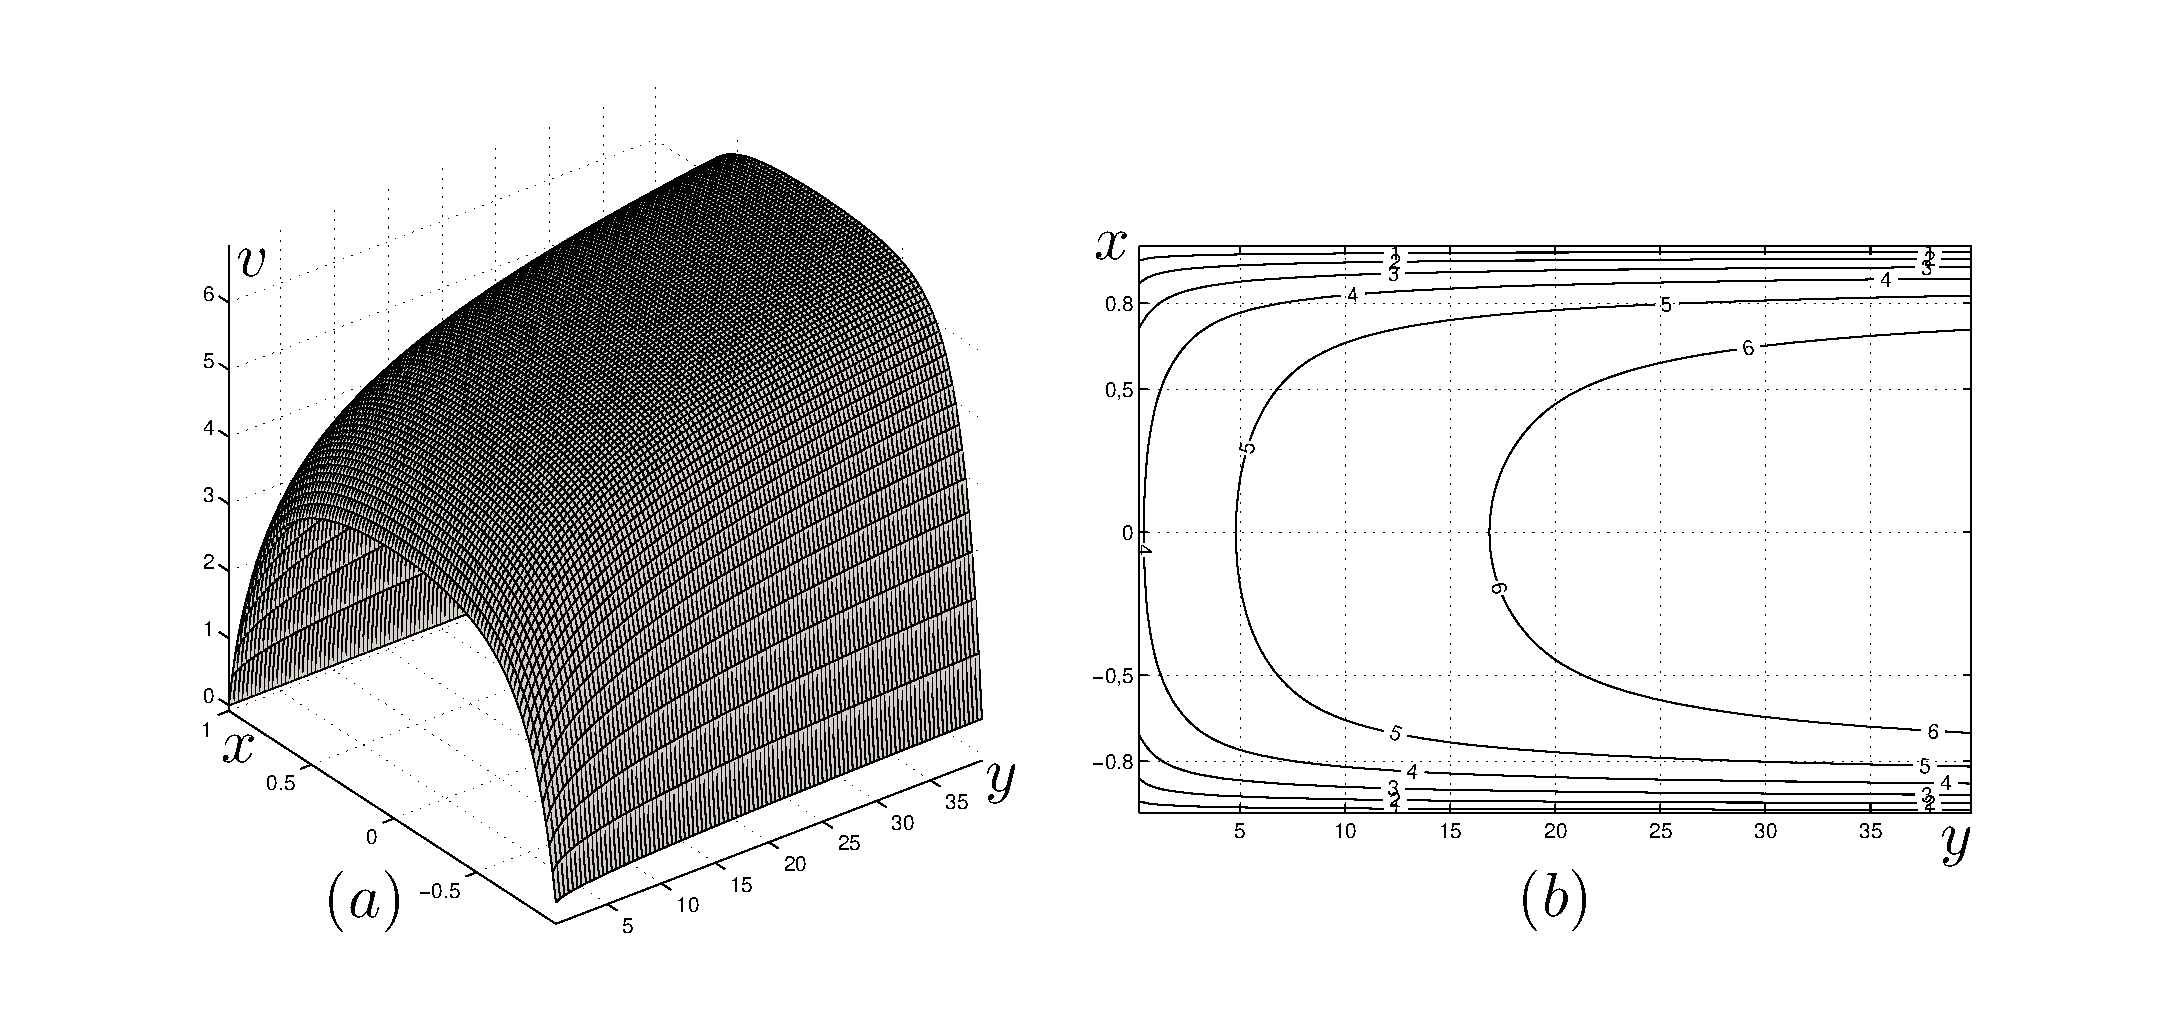
\includegraphics[width=1\textwidth]{v_last.eps}
         \caption{Функция Беллмана (a) и её линии уровня (b) при $k=2$.}
         \label{fig:2.1}
\end{figure}

Линии переключения оптимальных стратегий $\alpha^*$, соответствующие оптимальным значениям $a$ в (\ref{eq:2.3.3}), показаны на рис. \ref{fig:2.2}. Средняя область, содержащая точку равновесия, является областью бездействия $\Pi_{na}$, где $\alpha^*=0$. В ее дополнении имеем $\alpha^*=-10$ вблизи верхней границы $x=l$, и $\alpha^*=10$ вблизи нижней границы $x=-l$.

\begin{figure}[ht!]
      \centering
          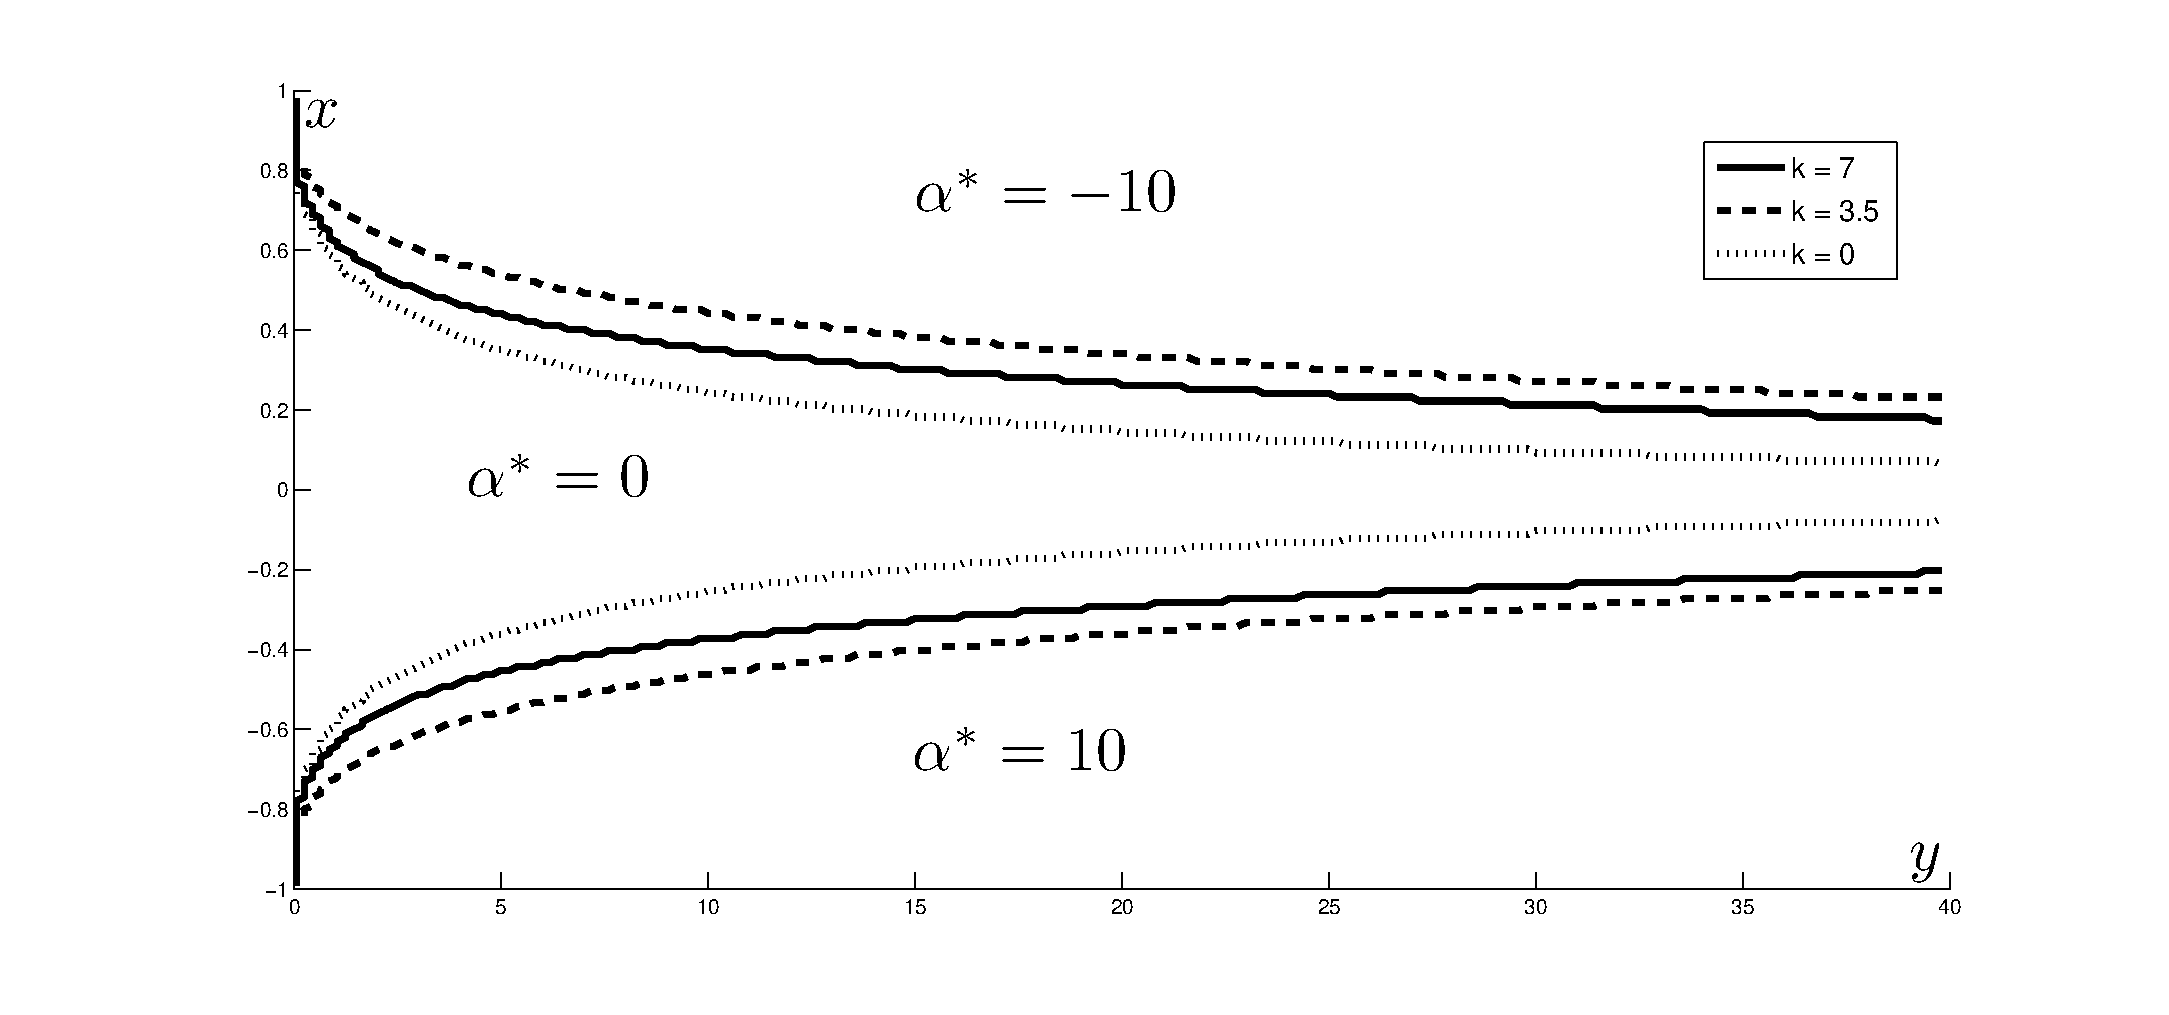
\includegraphics[width=1\textwidth]{control_mu.eps}
        \caption{Оптимальное управление в устойчивом случае.}
        \label{fig:2.2}
\end{figure}

Область бездействия расширяется при уменьшении $y$. Это означает, что регулятор становится менее активным, когда количество ресурса $Y$ уменьшается. Более интересный и неожиданный эффект касается <<немонотонного>> поведения области бездействия по отношению к $k$. Экспериментально было установлено, что $\Pi_{na}$ расширяется при увеличения $k$ от $0$ до $3.5$. Таким образом, регулятор менее вовлечен в процесс стабилизации системы, которая становится более устойчивой сама по себе. Но, для      $k>3.5$ наблюдается обратная картина: область бездействия сужается при дальнейшем увеличении $k$!

Заметим, что $v(x,y)$ определяет полезность текущего состояния $(x,y)$. Производные $v_x$, $v_y$ можно рассматривать как маргинальные полезности <<положения>> и <<топлива>>. Из рис. 3.1 ясно, что маргинальная полезность топлива убывает при увеличении количества топлива (т.е., $v$ вогнута по $y$). Маргинальная полезность положения положительна при $x\in (-l,0)$ и отрицательна при $x\in (0,l)$. Абсолютные значения $v_x$ малы вблизи $x=0$ и велики вблизи границ. Из (3.1) слеудет, что область бездействия $\Pi_{na}$ соответствует неравенству $v_y>|v_x|$, т.е., регулятор не потребляет топлива, когда маргинальная полезность последнего достаточно велика. Для малых $y$, с точки зрения регулятора, топливо стоит дорого, а значит область бездействия велика. Заметим также, что когда $k$ увеличивается ситуация становится более благоприятной, и $v_y$, $|v_x|$ должны стать меньше. Неясно, однако, как эти свойства влияют на поведение $\Pi_{na}$.

Оптимальные стратегии для неустойчивого случая $k<0$  представлены на рис. \ref{fig:2.3}. Здесь области бездействия значительно меньше. Это неудивительно, так как неустойчивую систему около точки равновесия удерживать сложнее. В противоположность устойчивому случаю, здесь $\Pi_{na}$ сжимается монотонно по $k$.
\begin{figure}[ht!]
        \centering
         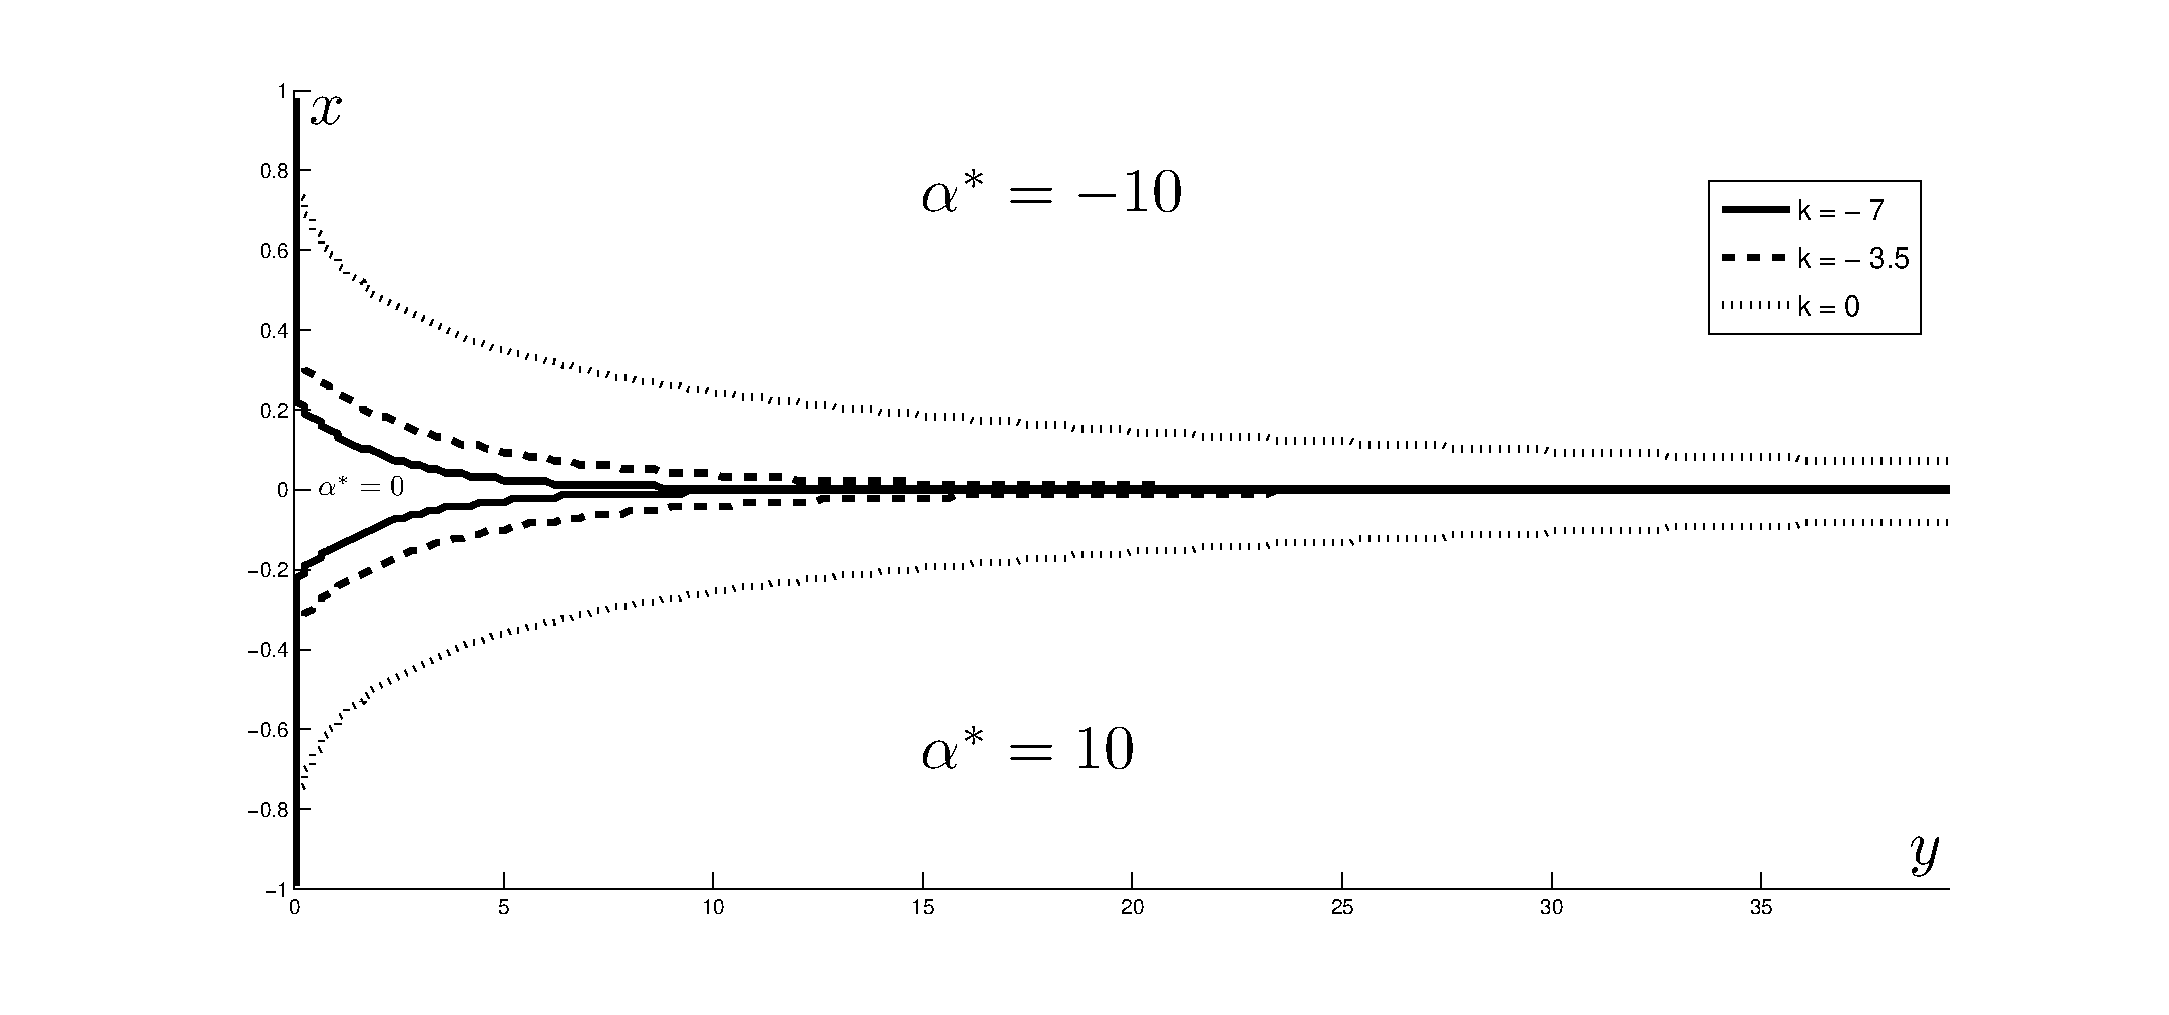
\includegraphics[width=1\textwidth]{control_minus_mu.eps}
        \caption{Оптимальное управление в неустойчивом случае.}
          \label{fig:2.3}
\end{figure}
Кроме того, функция Беллмана $v$ в этом случае меньше. Мы не приводим здесь график $v$, так он выглядит аналогично рис. \ref{fig:2.1}(a).

\section{Оптимальное отслеживание стохастической системы} \label{sec:2.4}
Рассмотрим случайную цель $X^1$, которую должен отследить управляемый процесс $X^2$. Флуктуации of $X^1$ описываются уравнением
\begin{eqnarray*}
dX^1_t &=& \mu(X^1_t) dt +\sigma dW_t,\quad \sigma>0,\\
\mu(x_1)&=& -k x_1 I_{\{|x_1|\le b\}} - k b I_{\{x_1\ge b\}}+k b I_{\{x_1\le -b\}},\quad b>0
\end{eqnarray*}
Случай $k>0$ (соотв., $k<0$) соответствует устойчивой (соотв., неустойчивой) точке равновесия $0$ соответствующей детерминированной системы. Динамика следящего процесса $X^2$, управляемого <<расходом топлива>>, не подвержена воздействию шума:
$$ dX^2_t =\alpha_t dt,\quad dY_t =-|\alpha_t|dt,\quad \alpha_t\in [\underline a,\overline a].$$
Предполагается, что слежение прекращается, если цель <<потеряна из виду>>:
$$\tau=\inf\{t\ge 0:|X^1_t- X^2_t|\ge l\},\quad l>0.$$

Для целевого функционала (\ref{eq:2.1.4}) уравнение HJB (\ref{eq:2.2.4}) принимает вид
$$ \beta v-1-\mu(x_1)v_{x_1}-\frac{1}{2}\sigma^2 v_{x_1 x_1}+\min_{a\in [\underline a,\overline a]}\{|a| v_y-a v_{x_2}\}=0,\quad
 (x,y)\in G\times (0,\infty), $$
где $G=\{x:|x_1-x_2|<l\}$. Граничные условия (\ref{eq:2.2.15}) преобразуются к следующей форме
$$ v=0\quad \textrm{на } \partial G\times [0,\infty);\quad v=\psi\quad \textrm{на } G\times\{0\},$$
где $\psi$ --- решение краевой задачи
\begin{eqnarray}
&&\beta \psi-1-\mu(x_1)\psi_{x_1}-\frac{1}{2}\sigma^2 \psi_{x_1 x_1}=0,\quad x_1\in (x_2-l,x_2+l),\label{eq:2.4.1}\\
&&\psi(x_2-l,x_2)=\psi(x_2+l,x_2)=0.\label{eq:2.4.2}
\end{eqnarray}

Проверим выполнение условий \ref{as:2.1}-\ref{as:2.3}. Пусть $\psi_1, \psi_2\in C^2(\mathbb R)$ --- система фундаментальных решений обыкновенного линейного дифференциального уравнения (\ref{eq:2.4.1}).Тогда
$$ \psi(x_1,x_2)=C_1(x_2)\psi_1(x_1)+C_2(x_2)\psi_2(x_1)+1/\beta, $$
где константы $C_1$, $C_2$ однозначно определяются граничными условиями (\ref{eq:2.4.2}). Отсюда следует, что $\psi\in C^2(G)$ и условие \ref{as:2.1} выполнено. Условие 2 выполняется, так как справедливо (\ref{eq:2.2.13A}). Для проверки условия \ref{as:2.3} достаточно показать, что функция $\psi$ и её производные до второго порядка включительно равномерно ограничены на $G$. Но это свойство следует из того факта, что при достаточно больших $|x|$ функция $\mu$ постоянна, $\psi=\varphi(x_1-x_2)$, где $\varphi(z)$ определяется следующим образом:
$$\beta \varphi-1-\mu\varphi_z-\frac{1}{2}\sigma^2 \varphi_{zz}=0,\quad z\in (-l,l);\quad \varphi(-l)=\varphi(l)=0.$$

Для численного решения задачи, как и в предыдущем примере, мы используем монотонную конечно-разностную схему:
\begin{eqnarray*}
 0&=&\beta v_{i,j,k} -1 -k\mu^+(x_{ijk})\frac{v_{i+1,j,k}-v_{i,j,k}}{h_1}+k\mu^+(x_{ijk})\frac{v_{i,j,k}-v_{i-1,j,k}}{h_1}\\
 &-&\sigma^2\frac{v_{i-1,j,k}-2v_{i,j,k}+v_{i+1,j,k}}{2 h_1^2} \\
 &+&\min_{a \in [\underline a,\overline a]}
 \left\{|a|\frac{v_{i,j,k}-v_{i,j,k-1}}{h_3}-a^+\frac{v_{i,j+1,k}-v_{i,j,k}}{h_2} +a^-\frac{v_{i,j,k}-v_{i,j-1,k}}{h_2}   \right\}, \quad x_{ijk}\in \Pi_h;\\
0&=&v_{ijk}-g(x_{ijk}),  \quad x_{ijk}\in \partial \Pi_h.
\end{eqnarray*}
Шаги $h_1$, $h_2$ выбраны таким образом, что точки сетки $x_{ijk}=(ih_1,jh_2,kh_3)$, $(i,j,k)\in \mathbb Z\times\mathbb Z\times\mathbb Z_+$ с $j=\max\{j':x_{ij'k}\in \Pi\}$ и $j=\min\{j':x_{ij'k}\in \Pi\}$, принадлежат $\partial\Pi$.
Сетка $\overline\Pi_h$ представляет из себя подмножество точек $\{x_{ijk}=(ih_1,jh_2,kh_3)\in\overline\Pi(r,\overline y):(i,j,k)\in \mathbb Z\times\mathbb Z\times\mathbb Z_+\}$, где множество $\overline\Pi(r,\overline y)=\{|x_1-x_2|\le l,\ |x_1+x_2|\le r,\ y\in [0,\overline y]\}$ вырезано из $\overline G\times [0,\infty]$. Значения $r$, $\overline y$ определяют искусственную границу. Как и в разделе \ref{sec:2.3}, через $\partial\Pi_h$ мы обозначаем те точки $\overline\Pi_h$, которые принадлежат границе множества $\Pi$. Другие точки сетки отнесены к $\Pi_h$.

Исследование данной схемы проводится аналогично разделу \ref{sec:2.3}. Сходимость ее решения $v_h$ к функции Беллмана $v$ вытекает из теоремы \ref{th:1} согласно методу Барля-Зуганидиса. Сеточная функция $v_h$ находится при помощи итераций (\ref{eq:2.3.7}). Начальные приближения $\underline v^0=0$, $\overline v^0= 1/\beta$, и критерий остановки остаются прежними.

Удобно сделать преобразование поворота
$$z_1=(x_1+x_2)/\sqrt 2,\quad z_2=(x_1-x_2)/\sqrt 2$$
и представить результаты в новых переменных $(z_1,z_2)$. Рассмотрим область $\{(z_1,z_2,y):z_1\in (-2,2), z_2\in (-40,40), y\in(0,10)\}$, соответствующую $l=4/\sqrt 2$, $r=80/\sqrt 2$, $\overline y=10$. В экспериментах были использованы следующие параметры: $\beta=0.1$, $\sigma=0.8$, $b=2.5$, $\overline a=-\underline a=1$. Сетка содержала $2000\times 100\times 50$ узлов. При $\varepsilon=0.01$ в (\ref{eq:2.3.8}) итерации обычно останавливались после 10 тысяч шагов.


Линии переключения оптимального управления в устойчивом ($k=0.3$)  и неустойчивом ($k=-0.3$) случаях показаны на рис.
\ref{fig:2.4} и \ref{fig:2.5} соответственно (при $y=1$).
\begin{figure}[h]
        \centering
       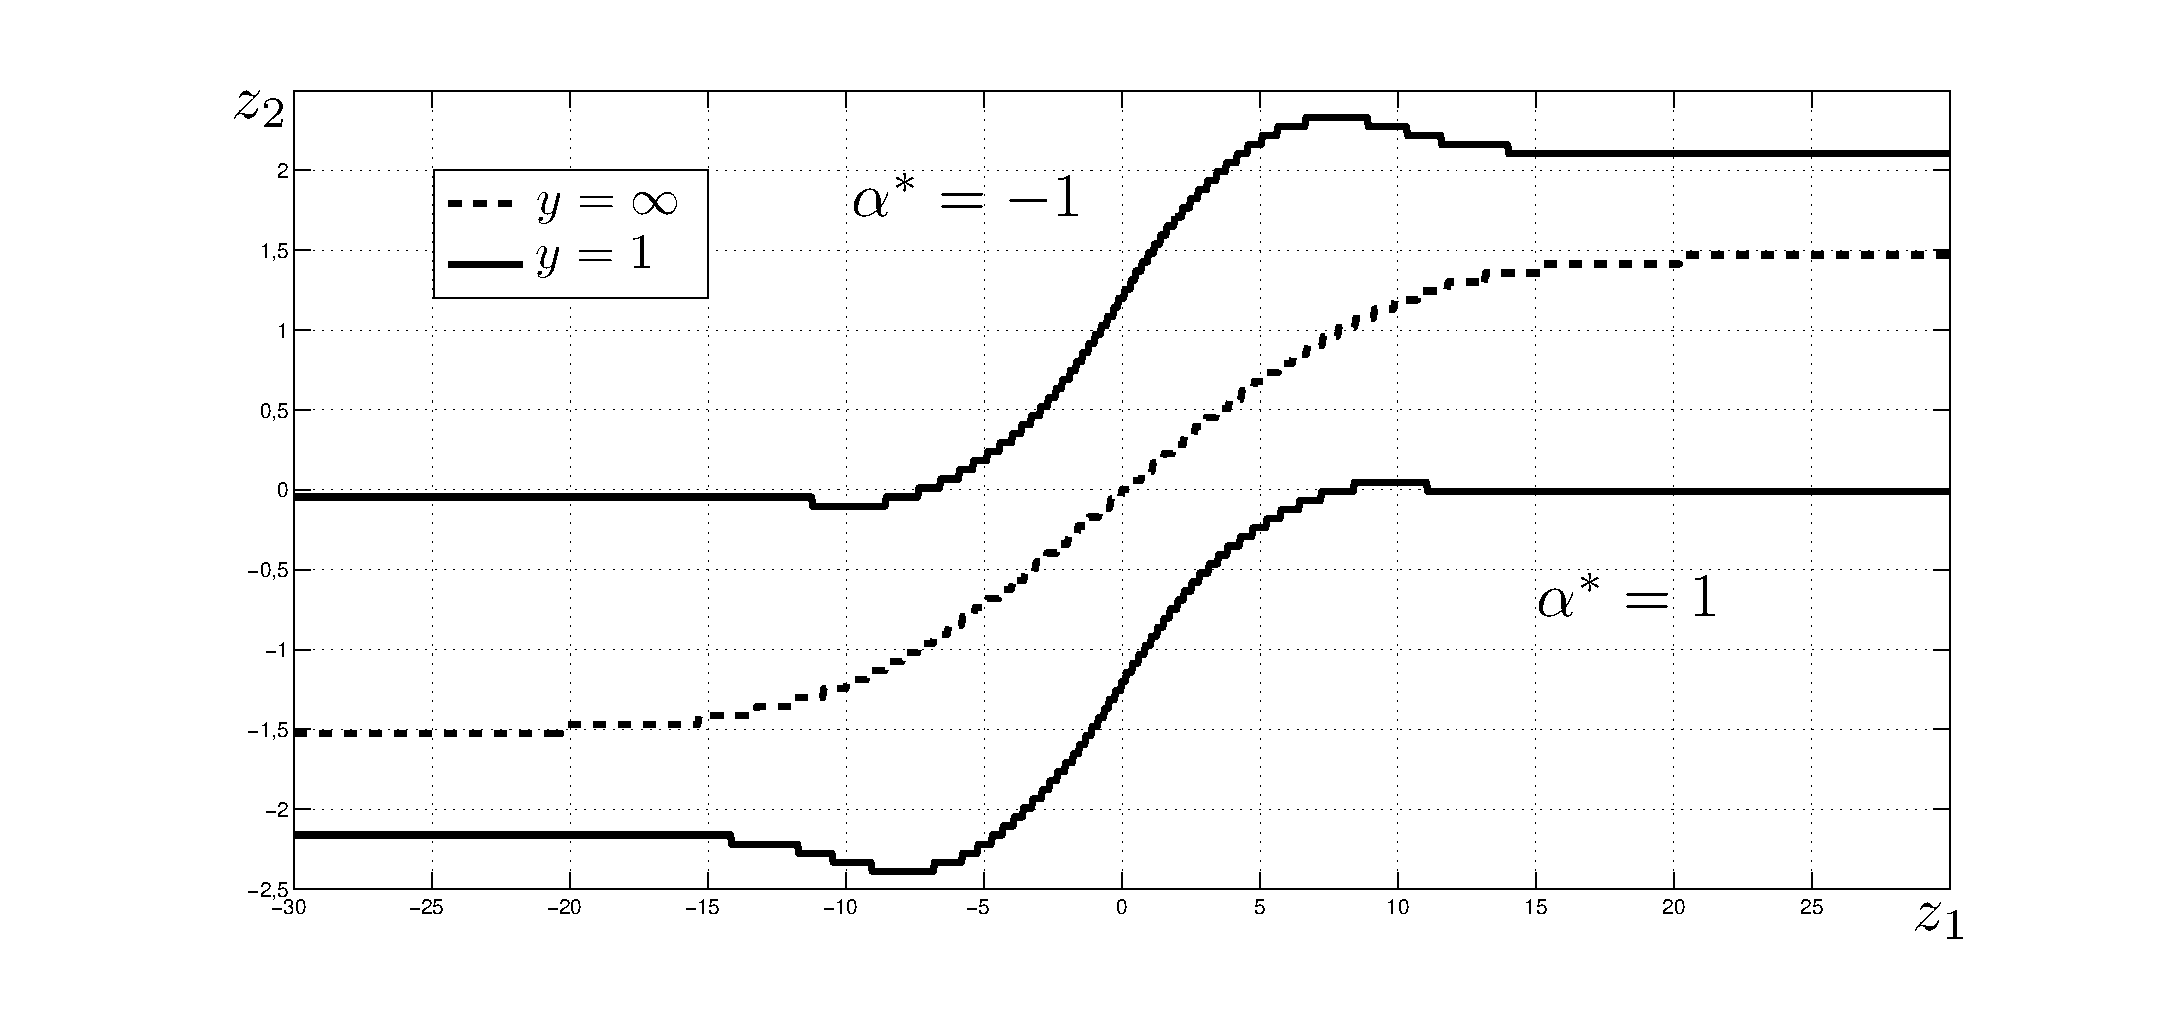
\includegraphics[width=1\textwidth]{u5_plus.eps}
         \caption{Оптимальное управление в устойчивом случае, $k=0.3$.}
         \label{fig:2.4}
\end{figure}
\begin{figure}[h]
        \centering
       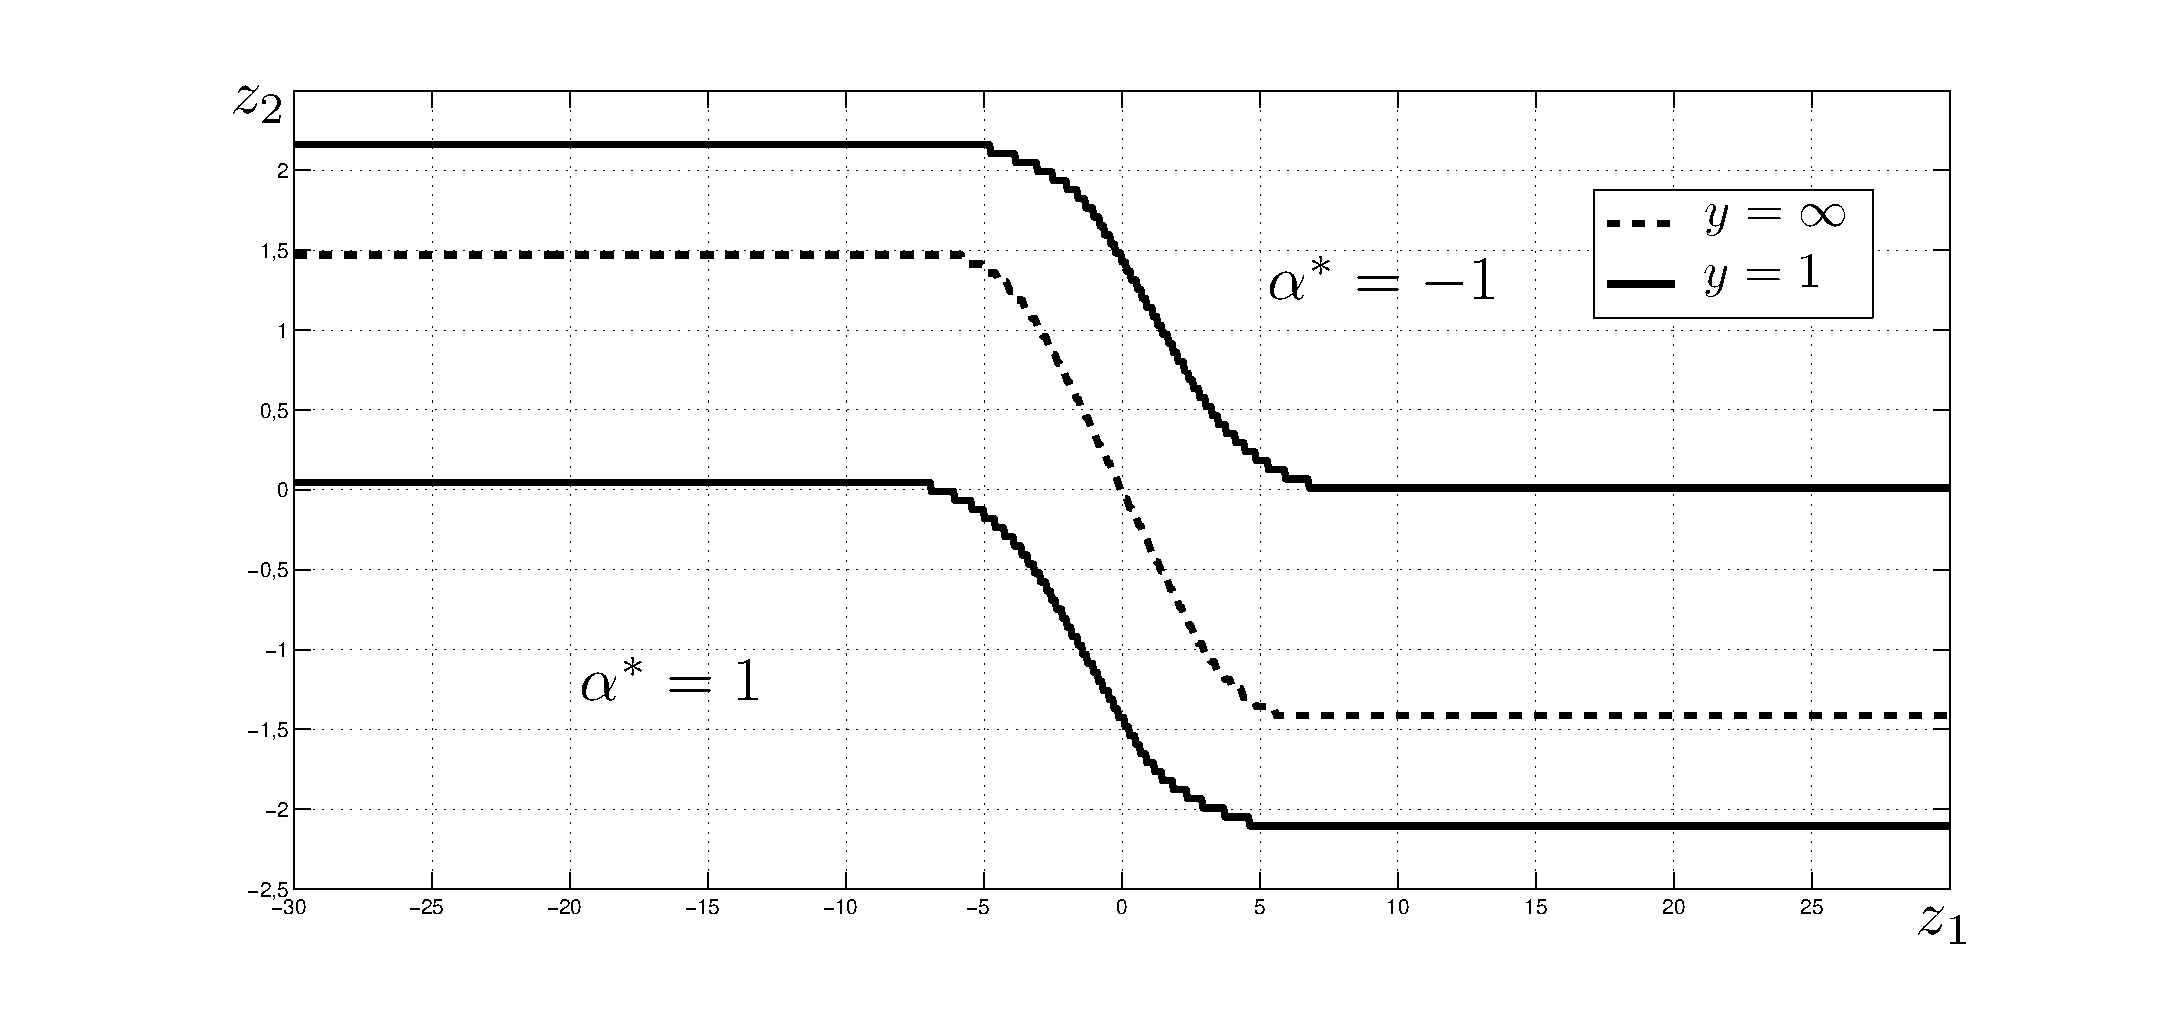
\includegraphics[width=1\textwidth]{u5_minus.eps}
         \caption{Оптимальное управление в неустойчивом случае, $k=-0.3$.}
         \label{fig:2.5}
\end{figure}

Области между сплошными линиями соответствуют множествам бездействия. Пунктирные линии определяют переключения оптимального управления для задачи (\ref{eq:2.2.12}), (\ref{eq:2.2.13}) с бесконечным топливом (здесь множества бездействия пусты).
Поскольку функция $\mu$ постоянна при $|x_1|>b$, линии переключения стабилизируются при достаточно больших  $|z_1|$. Кроме того, для больших $z_1>0$ область бездействия расположена выше (соотв., ниже) линии $z_2=0$ в устойчивом (соотв., неустойчивом) случае. Причина состоит в том, что в устойчивом случае, при $\alpha=0$, точка $(Z^1_t,Z^2_t)=(X_t^1+X_0^2,X_t^1-X_0^2)/\sqrt 2$ при больших $Z^1_0>0$, в среднем, движется от верхней границы полосы $(z_1,z_2)\in\mathbb R\times (-l,l)$ к ее нижней границе. В неустойчивом случае имеется противоположная тенденция. Для $z_1<0$ соответствующие картины могут быть получены при помощи отражения относительно начала координат.

Примеры графиков и линий уровня функций Беллмана $v$ в устойчивом и неустойчивом случаях представлены на рис. \ref{fig:2.6} и \ref{fig:2.7}.

\begin{figure}[h]
        \centering
       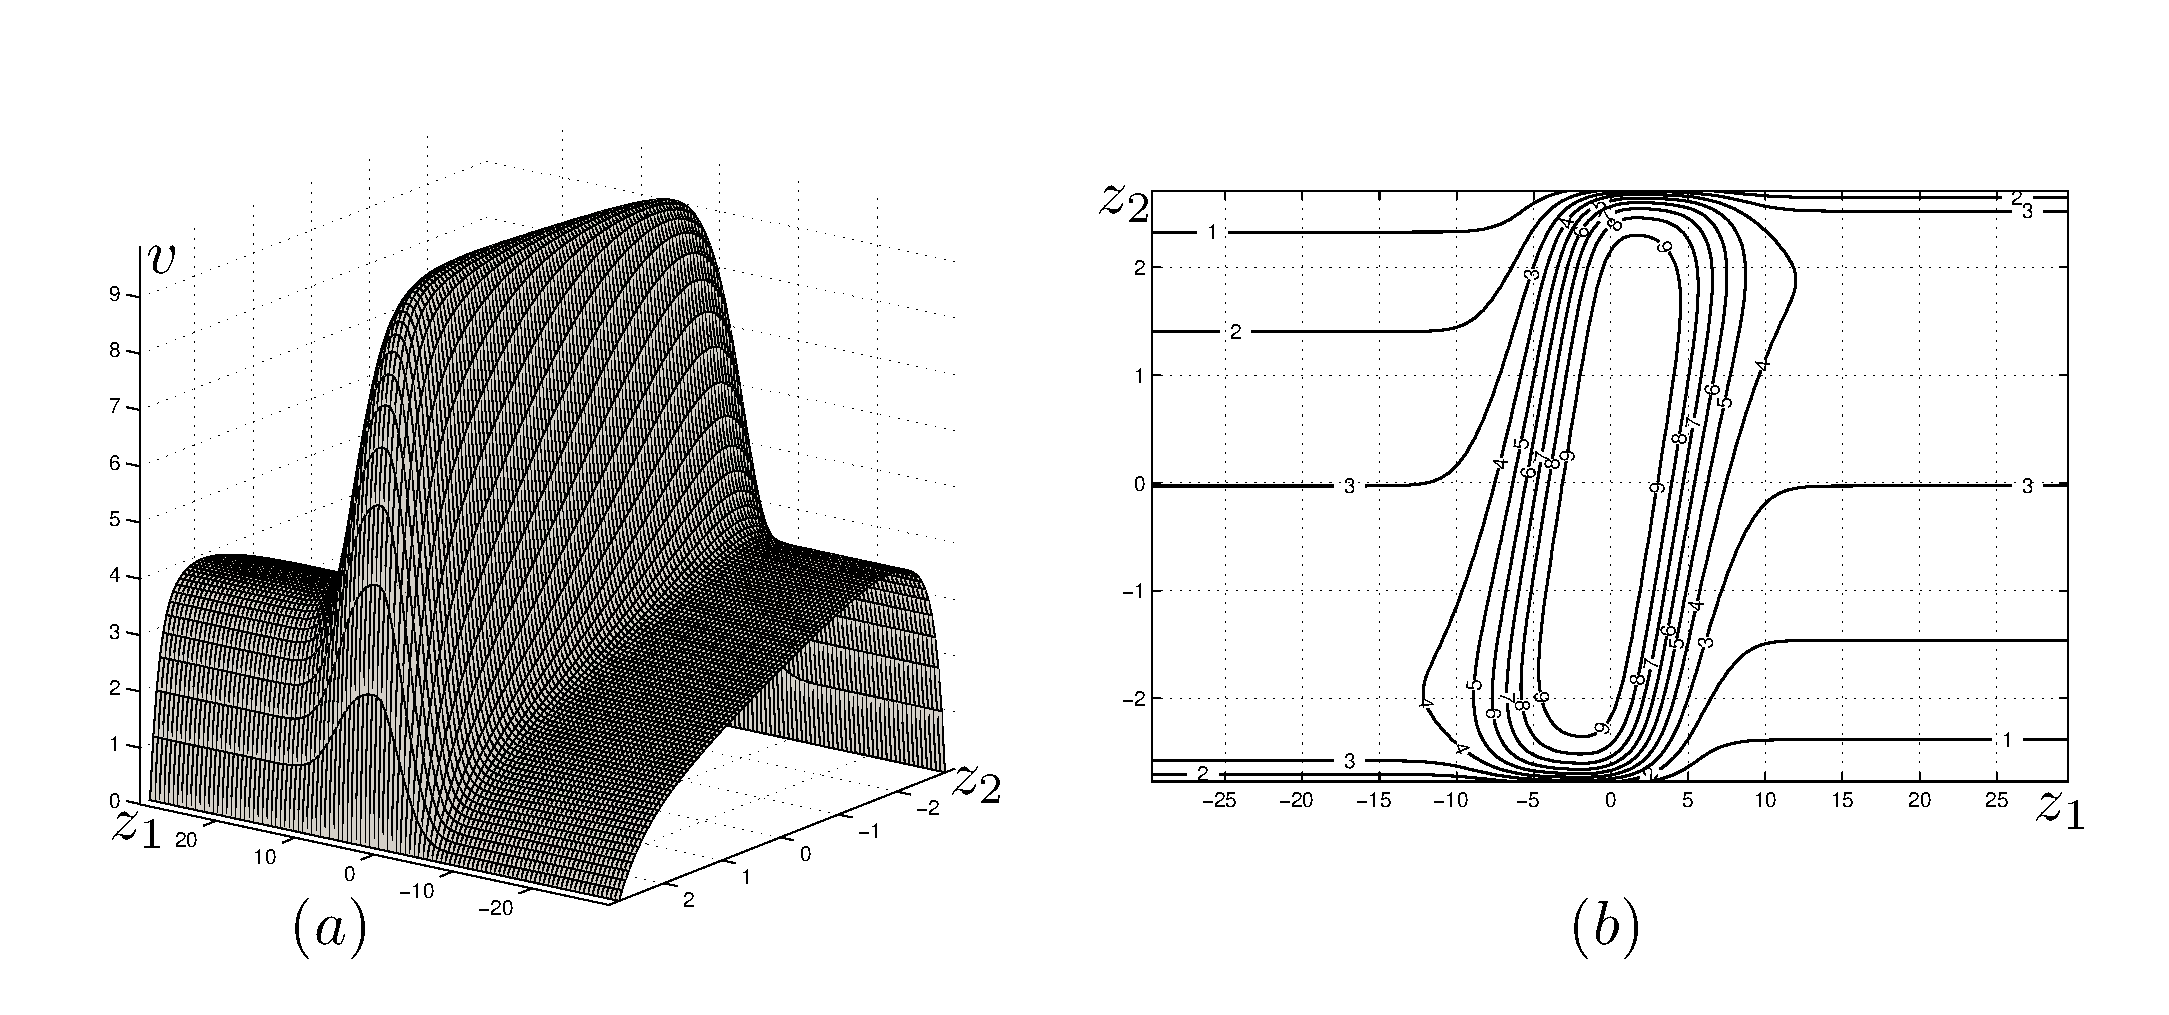
\includegraphics[width=1\textwidth]{v5_plus.eps}
         \caption{Функция Беллмана(a) и её линии уровня (b) при $k=0.3$.}
         \label{fig:2.6}
\end{figure}
\begin{figure}[h]
        \centering
       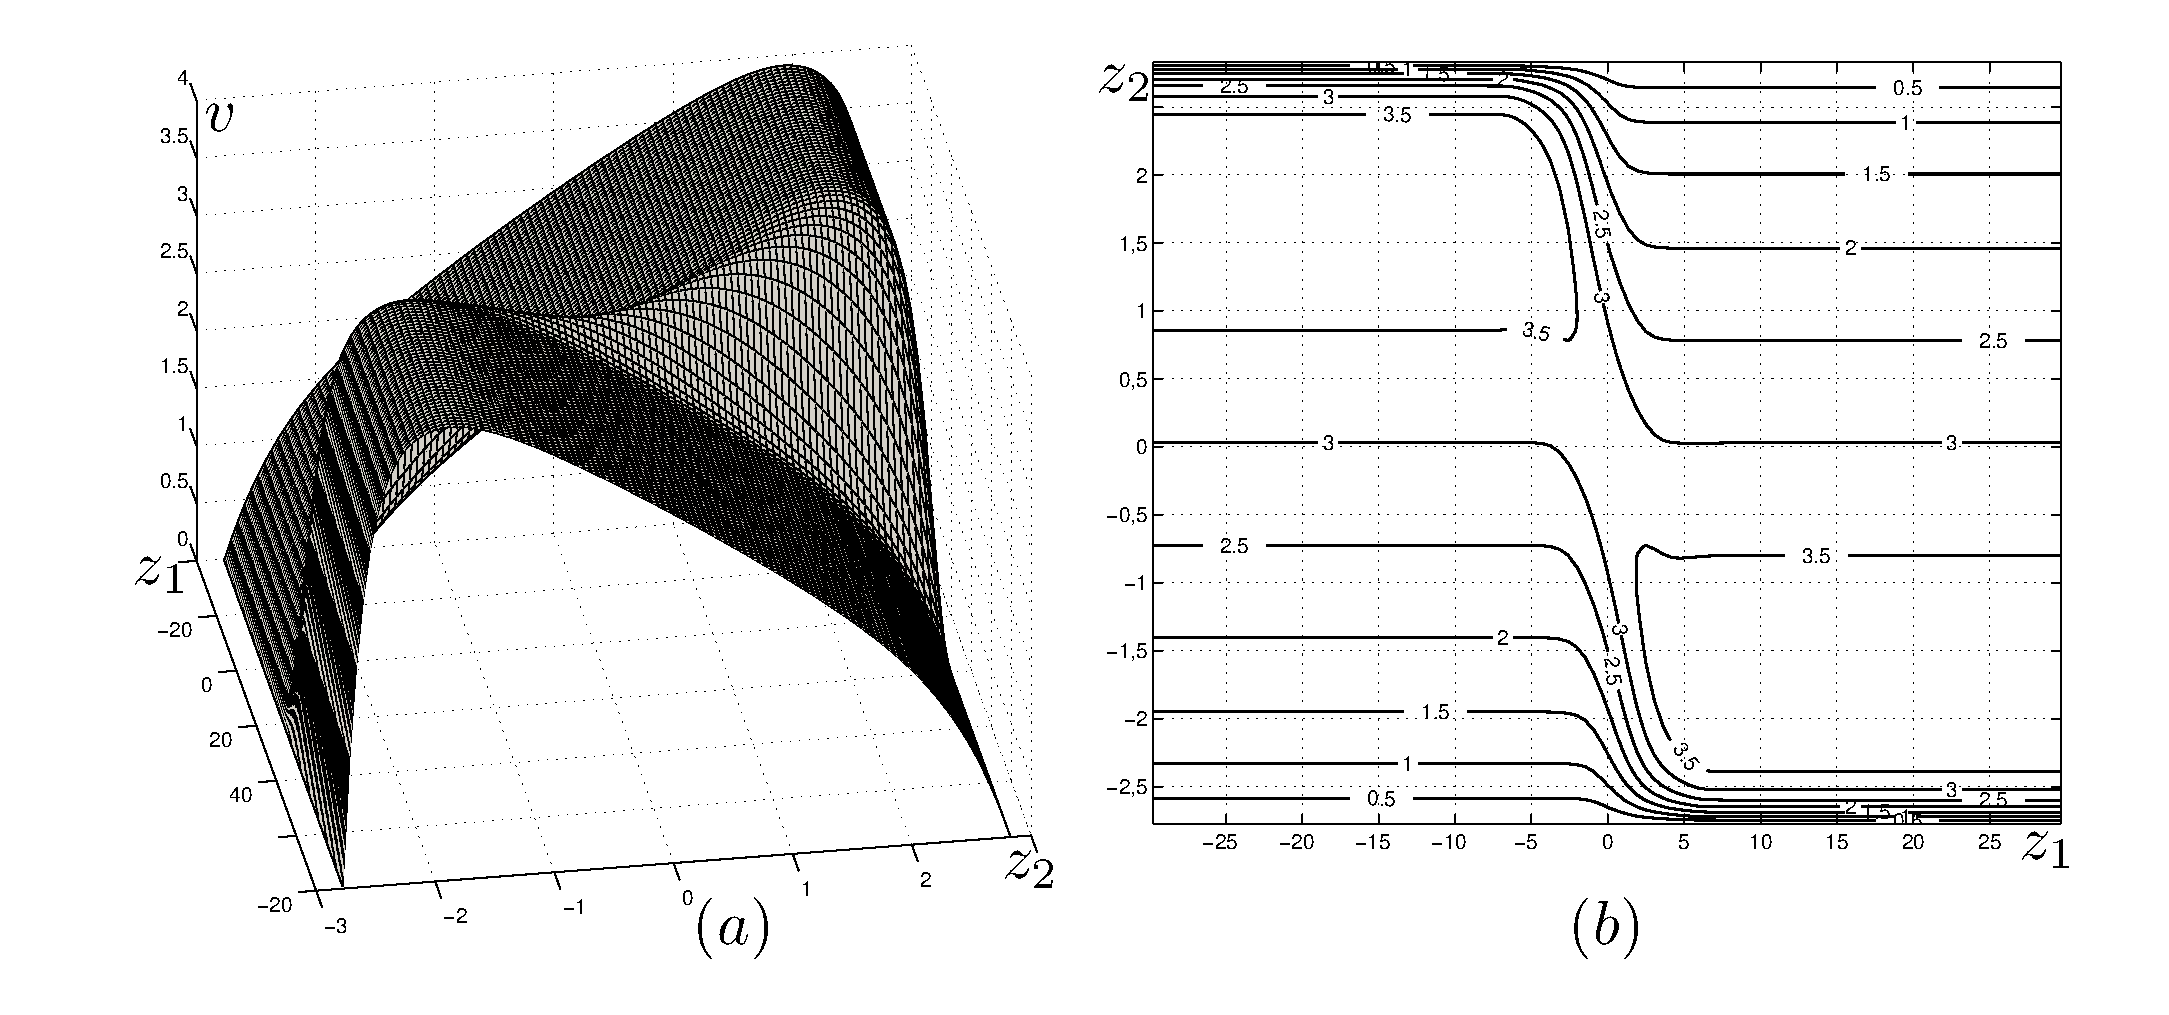
\includegraphics[width=1\textwidth]{v5_minus.eps}
         \caption{Функция Беллмана(a) и её линии уровня (b) при $k=-0.3$.}
         \label{fig:2.7}
\end{figure}

Для фиксированных $z_1, y$ функции Беллмана достигают своих максимумов по $z_2$ в областях бездействия. Глобальный максимум в устойчивом случае достигается в нуле. Однако, в неустойчивом случае, точки максимума функции $v$ расположены тех частях областей бездействия, где $|z_1|$ достаточно велико и $v$ почти константа по $z_1$.

\clearpage
